% This is the report Template for Fr. C Rodrigues Institute of Technology, Vashi

% Authored by -  Dr. Smita Dange

% Modularised every section into different .tex files

% This is the preamble.  

% Any package you would like to use, please add it to this .tex and not the other .tex files because if you do...the code will not compile! Other .tex files are only for filing content. Any styling has to happen in this file.

% Good Luck!
\documentclass[12pt]{report}
\usepackage{hyperref}
\usepackage{kantlipsum}
\usepackage{graphicx}
\usepackage{geometry}
\usepackage{ragged2e}
\usepackage{titlesec}
\usepackage{fancyhdr}
\usepackage{tabularx}
\usepackage{array}
\usepackage{float}
\usepackage{listings}
\usepackage{caption}
\usepackage{xcolor}
\usepackage{longtable}
\usepackage[table]{xcolor}
\usepackage{xltabular}
\usepackage{makecell}

\lstset{
    basicstyle=\ttfamily\footnotesize,
    breaklines=true,
    breakatwhitespace=false,
    frame=single,
    numbers=none,
    showstringspaces=false,
    keepspaces=true,
    columns=fullflexible,
    backgroundcolor=\color{gray!5},
    rulecolor=\color{gray!60},
    xleftmargin=0.3cm,
    xrightmargin=0.3cm,
    aboveskip=0pt,
    belowskip=0pt,
    lineskip=-1pt,
    tabsize=4,
    captionpos=t
}


\titleformat{\chapter}[display]
  {\normalfont\huge\bfseries\centering}
  {\chaptertitlename\ \thechapter}{24pt}{\Huge}
\geometry{verbose,a4paper,tmargin=15mm,bmargin=30mm,lmargin=30mm,rmargin=20mm}

%creating a user defined footer and header
\geometry{headheight=15pt}
\setcounter{tocdepth}{3}
\setcounter{secnumdepth}{3}

\pagestyle{fancy}
\fancyhf{}
\rhead{Project title}
\lfoot{F.C.R.I.T, Vashi}
\rfoot{\thepage}
\renewcommand{\footrulewidth}{0.6pt}
\renewcommand{\headrulewidth}{1.pt}
\usepackage[numbers]{natbib}

\begin{document}
\nocite{
  zhao2023,
  iman2021,
  jiang2025,
  abbadi2025,
  romsaiyud2025,
  lime,
  hybrid_recommender,
  mit_sop,
  cmu_admissions,
  cmu_sop_guidelines,
  mit_faculty_essay,
  scikit_learn,
  xgboost,
  huggingface_nlp,
  shap,
  google_recommendation,
  what_if_tool
}
\pagestyle{plain}
%Title Page

\begin{titlepage}
%%%% \pagenumbering{gobble}
\thispagestyle{empty}

{\centering
{A Project Report}\\ 
\vspace{0.2cm}
{On}
\vspace{0.4cm}
\\
}
 
{\centering
\large

{{\LARGE\bf MS-Admit : AI-Powered Admission Competitiveness and Profile Optimizer}\\[4pt]}\\
\vspace{1cm}
{Submitted in partial fulfilment of the requirements of } \\
\vspace{0.2cm}
{\bf{University of Mumbai}} \\
\vspace{0.2cm}
{For the Degree of} \\
\vspace{0.2cm}
{\bf {Bachelor of Technology }} \\
{\it{in}} \\
{\bf COMPUTER ENGINEERING } \\
\vspace{0.5cm}
\it{Submitted by} \\
\vspace{.2cm}
\rm
{\large \bf {Samiksha Khandagale }}\\
{\large \bf {Shivangi Khandelwal }}\\
{\large \bf {Shubham Khilari}}\\
{\large \bf {Racheal Kodiyan}}\\

\vspace{1.2cm}
{\it{Supervised by}} \\
\vspace{.2cm}
\hspace{.05cm} {\large \textbf {Dr.Chhaya Pawar}}\\
\vspace{0.2cm}



\begin{figure}[h]
{\centering {
\includegraphics[width=4cm,height=4cm]{fcritlogo}}\par}
\end{figure}

{\bf Department of Computer Engineering \\
\vspace{0.2cm}
\bf {Agnel Charities',Fr. Conceicao Rodrigues Institute of Technology}\\
{\small\bfseries (An Autonomous Institute & Permanently Affiliated to University of Mumbai)}
\bf Sector 9A, Vashi, Navi Mumbai - 400703} \\
{\centering
\hspace{.5cm}


{\centering
{\bf UNIVERSITY OF MUMBAI} \\

\bf{2026-2027} \\
}

}\end{titlepage} 
\pagenumbering{roman}


%\pagenumbering{gobble}


% Approval Page 

\begin{center}

{\LARGE\bf APPROVAL SHEET}

\vspace{0.8cm}

{\large This is to certify that the project entitled}\\[0.3cm]

{\Large\bf \textsc{``MS-Admit : AI-Powered Admission Competitiveness and Profile Optimizer''}}\\[0.4cm]

{\large\bf Submitted by}\\[0.4cm]

\begin{table}[h]
\centering
\Large
\begin{tabular}{cc}
\textbf{Samiksha Khandagale} & \textbf{1023151} \\
\textbf{Shivangi Khandelwal} & \textbf{1023152} \\
\textbf{Shubham Khilari} & \textbf{1023153} \\
\textbf{Racheal Kodiyan} & \textbf{1023154}
\end{tabular}
\end{table}

\vspace{0.8cm}

{\large
In partial fulfilment of degree of B.Tech (Semester VII) in Computer
Engineering for continous assessment  of Major project is approved.
\par
}

\vspace{1.2cm}

%------------------------------------------------
% Signature Sections
%------------------------------------------------

\begin{raggedleft}
\large{\textbf{Supervisor(s) :  \rule{8cm}{0.2px}}} \\ [1cm]
\large{\textbf{Project Coordinator(s) : \rule{5.7cm}{0.2px}}} \\ [1cm]
\large{\textbf{Examiners  : 1. \rule{8cm}{0.2px}}} \\ [1cm]
\large{\textbf{2. \rule{8cm}{0.2px}}} \\ [1cm]
\large{\textbf{Head of Department : \rule{6cm}{0.2px}}} \\ [3cm]
\end{raggedleft}
\begin{flushleft}
\textbf{Date : }\\[0.2cm]
\textbf{Place : Navi Mumbai} 
\end{flushleft}
%------------------------------------------------
% College Seal
%------------------------------------------------

\textbf{COLLEGE SEAL}

\vspace{1.8cm}

\end{center}

% Declaration Page

\begin{centering}
\large
{\LARGE\bf Declaration}\\
\end{centering}

% workaround for the inconsistent justify. If someone figures out the right way to strictly justify, let me know
\justify
We declare that this written submission for B.E. Declaration entitled 
"{\bf MS-Admit : AI-Powered Admission Competitiveness and Profile Optimizer}" represents our ideas in our own words and where others' ideas or words have been included. We have adequately cited and referenced the sources. We also declare that we have adhered to all principles of academic honesty and integrity and have not misrepresented, fabricated, or falsified any ideas/data/fact/source in our submission. We understand that any violation of the above will cause disciplinary action by the institute and also evoke penal action from the sources which have thus not been properly cited or from whom permission has not been taken when needed.  \\ 

\vspace{3cm}
\hfill% move it to the right
\begin{tabular}[t]{l@{}}
\vspace{1cm}

{\textbf{Project Group Members:}} \\ 
\vspace{1cm}

1. Samiksha Khandagale, 1023151\\
\noindent\rule{5cm}{0.10pt} \\
\\
\vspace{1cm}

2. Shivangi Khandelwal, 1023152 \\
\noindent\rule{5cm}{0.10pt} \\
\\
\vspace{1cm}

3. Shubham Khilari, 1023153 \\
 \noindent\rule{5cm}{0.10pt}
\\
\vspace{1cm}

4. Racheal Kodiyan, 1023154 \\
 \noindent\rule{5cm}{0.10pt}
\\
\vspace{1cm}
\end{tabular}

%%%%%%%%%%%%%%%%%%%%%%%%%%%%%%%%%%%%IGNORE PLEASE !
%\begin{flushright} 
%\vspace{0.5in}
%\noindent\rule{4cm}{0.4pt} \\ (Signature)\\
%\vspace{0.3in}
%\noindent\rule{4cm}{0.4pt} \\ (Name of the Student)
%\end{flushright}
%\vspace{0.5cm}
%{\bf Date:} \\
%%%%%%%%%%%%%%%%%%%%%%%%%%%%%%%%%%%%


%% End of Declaration Page


% Table of Contents
\newpage

%Abstract
\addcontentsline{toc}{chapter}{Abstract}
% Abstract Page
\vspace{1in}
\chapter*{Abstract}

\justify
Graduate admissions requires a challenging decision; as the requirements can be different, as well as the backgrounds of the students, and as a result of admission standards, acceptance criteria is different. Nowadays, most university recommendation platforms use QS rankings or generic suggestions, which means they provide very little personal help or detailed explanations. This article highlights MsAdmit a framework to analyze data that aids in the decision making process and develop unique ways to prepare and apply for graduate applications, specifically for Master’s in Computer Science programs. A system that is being recommended uses machine learning and big language models to look for applicant profiles. These profiles come from information such as GPA, scores from standard tests, previous research experience, work experience in industries, and the degree of the current undergraduate institution. It predicts how likely something is to be adopted and employs explainable AI tools, such as SHapley Additive exPlanations (SHAP), to understand the key elements in a profile and areas for further enhancement. It breaks universities(Top 150 QS ranked) down into 3 different categories – Target, Consider, and Reach, per type of applicant and institution. Also, an underlying “what-if” simulation can help applicants see how differences in test scores and elements of their profile could affect their estimate of a successful student. Such a system enables students to make their choices obvious and using data, providing simple suggestions, and continually updating admissions information. By simplifying profile assessment, explaining decision-making, college suggestions, and customized plans into one system, it makes it easier and more user-friendly for students to handle the process of getting graduated. An accurate prediction with good recommendation should not be an undone fact, due to past admission data, to test this concept as accurately and effectively as possible.


\vspace{25pt}
\textbf{Keywords:} Graduate admissions, QS Rankings, Explainable Artificial Intelligence (XAI), Machine learning, SHapley Additive exPlanations (SHAP), Large Language Models (LLMs), University recommendation, Admission competitiveness, Decision-support systems.

\tableofcontents
\newpage

\addcontentsline{toc}{chapter}{List of Figures}
\listoffigures
\newpage

\addcontentsline{toc}{chapter}{List of Tables}
\listoftables
\newpage

\newpage

\pagenumbering{arabic}

\pagestyle{fancy}
% Chapter 1 Introduction
\fancyhead[R]{\small MsAdmit}
\chapter[Introduction]{\centering Introduction}\label{chap1}
\newpage

\section{Background}
\justify

Applying for a Master's program abroad is one of the biggest academic decisions a student makes, and also one of the most uncertain. Applicants have to weigh their GPA, GRE and TOEFL/IELTS scores, work experience, internships and research publications against hundreds of universities, each with its own unwritten expectations. Most students rely on forums, consultants or word of mouth, which tends to be generic, inconsistent and often expensive. Few applicants can tell where their profile actually stands, which universities are realistic targets, or what to improve before the deadline.
 
Machine Learning, Explainable AI and Large Language Models make a more personal and transparent approach possible. MsAdmit is a full-stack platform that evaluates a student's profile and predicts their competitiveness for universities worldwide. It uses trained ML models (XGBoost and a stacking ensemble) on historical admission data, and SHAP explains each prediction so the student can see why a university is labelled Reach, Target or Consider. Resumes are uploaded as PDFs and parsed automatically into the metrics the models need. Google Gemini reviews Statements of Purpose against an 8-criteria rubric. A what-if simulator and strategic roadmap then show how improvements such as a GRE retake or a new publication would change the outcome.
\section{Motivation}
\justify

Students applying abroad face a gap between what they know and what they need to know. They often do not know how competitive they are, so they apply too high, too low, or without a clear strategy. Each application also carries real costs: fees, documents (SOP, three LORs, transcripts, resume) and deadlines that are easy to lose track of.
 
Existing tools mostly give a bare ``chance of admit'' number with no reasoning, or generic advice that ignores the individual profile. Students are left without answers to the questions that matter: why was this university placed in this category, and what should I do next?
 
MsAdmit was built to close that gap. It combines prediction with explanation and action. The student gets a competitiveness score, a clear breakdown of the factors behind it, feedback on their SOP, and a plan for improving their profile, all in one place alongside an application tracker.
\section{Aim and Objective}
\subsection*{Aim :}
\justify
MsAdmit aims to provide an efficient system of applying university to get a deeper insight into a person's profiles and discover optimal universities for graduate education. It delivers personalized advice to their admission applicants, assesses entry competitiveness, and recommends ways to improve, and that's how it allows a student to plan the next step towards their admission journey.

\subsection*{Objectives :}

The objective of MsAdmit is to create an AI-powered graduate
admissions decision support and profile optimization platform
that provides transparent, personalized, and actionable guidance
through a unified system. The detailed objectives of the project
are as follows:

\begin{itemize}
    \item To predict a student's competitiveness score from academic and profile data (GPA, GRE, TOEFL/IELTS, undergraduate tier, work experience, internships and publications) using machine learning models.
    \item To recommend universities in three tiers (Reach, Target and Consider) based on model inference and historical admission benchmarks.
    \item To apply Explainable AI (SHAP) so students can see which factors raised or lowered each prediction.
    \item To extract profile metrics automatically from uploaded PDF resumes and feed them into the prediction pipeline.
    \item To evaluate Statements of Purpose with Google Gemini against an 8-criteria \cite{mit_sop,cmu_admissions,cmu_sop_guidelines,mit_faculty_essay}rubric, with paragraph-level strengths and weaknesses.
    \item To provide an interactive what-if simulator and roadmap that shows the effect of GRE retakes, new publications or a stronger SOP.
    \item To provide an application tracker for documents, deadlines, notes and fee budgeting.
    \item To offer a QS Top 150 explorer with admission requirements, tuition and acceptance statistics.
    \item To build the system as a secure, scalable web application with a React frontend and a FastAPI backend, using JWT authentication and database support for MongoDB and SQL.
\end{itemize}


% \section{Problem statement}

% \section{Scope}


\section{Report Outline}


This report is organized into six chapters:

\begin{itemize}
    \item \textbf{Chapter 1: Introduction} presents the project background, problem statement, motivation, and objectives.

    \item \textbf{Chapter 2: Study of the System} reviews existing systems, related research, and their limitations.

    \item \textbf{Chapter 3: Proposed System} describes the MsAdmit platform, its key features, and workflow, including admission prediction, university recommendations, SOP evaluation, and profile optimization.

    \item \textbf{Chapter 4: Design of the System} explains the system architecture, data flow diagrams, database design, and machine learning methodology.

    \item \textbf{Chapter 5: Result and Discussion} presents the implementation results, model performance, system evaluation, and limitations.

    \item \textbf{Chapter 6: Conclusion \& Future Scope} summarizes the project's contributions and discusses potential future enhancements.
\end{itemize}



%%%% End of Chapter 1

% Chapter 2: Literature Survey

\chapter{Study of the System}
\fancyhead[R]{MsAdmit}
\newpage
\label{chap2}

\section{About the Technique}

Some students who attend the University admission are assessed on several criteria including academic performance, standardized test scores, research experience, internships, and personal documents (Student Statements of Purpose (SOP) and Letters of Recommendation (LOR). Conventional admission decisions were made manually and that were based on academic or research results. Although this approach allows for human judgment, it can become time-consuming and oftentimes create incorrect evaluations based on the number of applications requested. While introducing artificial intelligence (AI) and machine learning (ML), some parts of this process can be automated through collecting applicant data and evaluating patterns in previous admission results. Analysis methods of classification and prediction models may estimate the admission competitiveness of an applicant and analysis of SOPs, LORs and resumes using Natural Language Processing (NLP). Explainable AI (XAI) strategies can enable users to visualize what factors dictate a prediction. MsAdmit leverages these methods in order to assist students in making the evaluation of their profiles, compare their qualifications with university requirements, and identify learning opportunities. The system would rather support admission planning and decision making than eschew official university admission decisions.

\section{Various Available Techniques}

Different kinds of AI approaches can be employed in identifying and determining candidate profile data.

\
\begin{enumerate}

    \item \textbf{Machine Learning Classification and Prediction}

    Machine learning algorithms such as Logistic Regression, Random Forest, Support Vector Machine (SVM), and XGBoost can be used to estimate admission competitiveness based on applicant features such as GPA, test scores, research experience, and internships \cite{scikit_learn,xgboost}.

    \item \textbf{Natural Language Processing (NLP)}

    NLP techniques process unstructured text from resumes and other application documents to extract relevant information, identify skills, and support applicant profile evaluation \cite{huggingface_nlp}.

    \item \textbf{Explainable Artificial Intelligence (XAI)}

    XAI techniques such as SHAP and LIME help explain model predictions by identifying influential features, allowing applicants to better understand their strengths and areas for improvement \cite{shap,lime}.

    \item \textbf{Recommendation Systems}

    Recommendation techniques compare applicant profiles with relevant university information to suggest suitable institutions. Based on estimated competitiveness, universities can be grouped into Target, Consider, and Reach categories to support application planning \cite{google_recommendation}.

    \item \textbf{What-If Analysis and Profile Optimization}

    What-if analysis enables applicants to explore how changes in profile attributes may affect predicted outcomes, helping them identify potential areas for improvement. Such estimates are indicative and do not guarantee admission \cite{what_if_tool}.

    \item \textbf{Hybrid AI Techniques}

    Hybrid AI approaches combine multiple methods to improve the overall recommendation process. In MsAdmit, machine learning, NLP, explainability, and recommendation techniques work together to support admission competitiveness estimation and personalized profile improvement \cite{hybrid_recommender}.

\end{enumerate}


\section{Related Works}

Several authors have developed methods using Machine Learning, Natural Language Processing and Explainable AI in universities to predict the admission and assessment of students profiles. Research to do at the present paper MsAdmit provided these details of information from this symposium.


\subsection{A Machine Learning Approach to Graduate Admissions and the Role of Letters of Recommendation}

The study by Zhao et al. \cite{zhao2023} investigates the use of
structured academic information and recommendation-letter features
to predict graduate admission-related outcomes. The approach uses
IBM Watson Natural Language Understanding to analyze textual
information and SHAP to explain model predictions. The study reports
an accuracy of 89\%.

\noindent\textbf{Limitations / Gaps}
\begin{itemize}
    \item The study focused on a single university and two academic programs.
    \item Recommendation letters required manual rating, limiting automation.
    \item Precision, recall, and F1-score were not reported.
    \item Data sharing was restricted due to privacy requirements.
\end{itemize}

The study demonstrates the potential of combining structured academic
data, textual analysis, and explainable Machine Learning for admission
prediction. However, its limited institutional scope and reliance on
manual evaluation restrict generalizability. MsAdmit builds on this
approach by integrating automated document analysis, explainable
predictions, and university recommendations.

\subsection{A Comparison of Classification Models in Predicting Graduate Admission Decision}

Iman and Tian \cite{iman2021} compared several Machine Learning
algorithms using the Kaggle Graduate Admissions dataset. The
algorithms included Naive Bayes, Logistic Regression, Multilayer
Perceptron, Random Forest, and decision-tree-based models. The study
reported that Naive Bayes performed best and identified CGPA and
TOEFL scores as important predictors of admission outcomes.

\noindent\textbf{Limitations / Gaps}
\begin{itemize}
    \item The dataset contained only 400 records, limiting the reliability
    of broader conclusions.
    \item The data primarily represented Indian applicants, restricting
    geographical diversity.
    \item The study focused on structured numerical features.
    \item Explainability and fairness were not explored.
\end{itemize}

This research demonstrates the usefulness of academic performance
and standardized test scores in admission prediction. However, its
limited dataset and focus on numerical attributes leave scope for
more comprehensive applicant evaluation. MsAdmit extends this
approach by incorporating document analysis, explainable predictions,
and personalized university recommendations.

\subsection{Artificial Intelligence Use in Academic Applicant Screening: A Systematic Review}

Jiang et al. \cite{jiang2025} conducted a systematic review of research
on AI-based admission prediction, covering 18 studies involving
61,327 applicants. The review compared traditional Machine Learning
methods with Natural Language Processing techniques. According to
the conference paper, traditional Machine Learning methods achieved
an average AUROC of 0.89, compared with 0.77 for NLP approaches.

\noindent\textbf{Limitations / Gaps}
\begin{itemize}
    \item The reviewed studies used different datasets and evaluation
    methods, limiting direct comparisons.
    \item Only nine studies reported AUROC values.
    \item Statistical significance testing was not performed.
    \item Bias was identified as a concern in approximately half of the
    reviewed studies.
\end{itemize}

This review highlights the importance of selecting suitable prediction
techniques and evaluating their performance consistently. It also
emphasizes the need to address fairness, data quality, and
methodological limitations in AI-based admission systems. MsAdmit
considers these aspects through model evaluation, explainability, and
applicant profile analysis.

\subsection{LLM-Augmented and Fair Machine Learning Framework for University Admission Prediction}

Abbadi et al. \cite{abbadi2025} investigated university admission
prediction using four datasets and simulated personal-statement
scores generated with GPT-4. The study compared Logistic Regression,
Naive Bayes, Random Forest, Deep Neural Networks, and a stacked
ensemble. The ensemble reportedly achieved an accuracy of 91\%.
The researchers also examined fairness using demographic parity
and equalized odds.

\noindent\textbf{Limitations / Gaps}
\begin{itemize}
    \item Personal-statement scores were simulated rather than obtained
    from real admission evaluations.
    \item Validation using actual admission outcomes was limited.
    \item Implementation details and train-test split procedures were
    not sufficiently reported.
    \item Differences associated with gender and parental education
    were identified.
\end{itemize}

The study demonstrates the potential of combining multiple prediction
models with large language models and fairness evaluation. However,
the use of simulated statement scores and limited real-world
validation presents challenges for practical application. MsAdmit
builds on this direction by integrating applicant profile prediction,
statement-of-purpose evaluation, and explainability while recognizing
the importance of fairness assessment.

\subsection{Explainable AI Framework for Multiclass University Recommendations Using SHAP and Counterfactual SHAP}

Romsaiyud \cite{romsaiyud2025} explored an explainable university
recommendation approach using six Machine Learning models. XGBoost
achieved a reported accuracy of 88.69\%. SHAP and Counterfactual
SHAP were employed to explain predictions and identify changes in
applicant scores that could influence recommendation outcomes.

\noindent\textbf{Limitations / Gaps}
\begin{itemize}
    \item The study focused on Thai universities and the Computer
    Engineering discipline.
    \item Model implementation and train-test evaluation details were
    not fully specified.
    \item Evaluation across international universities was not reported.
\end{itemize}

This work is particularly relevant to MsAdmit because it combines
university recommendations with explainable predictions. However,
its restricted geographical and disciplinary scope limits its
applicability to diverse international applicants. MsAdmit extends
this approach by aiming to recommend universities across a broader
range of institutions and help students understand their predicted
competitiveness and identify areas for profile improvement.







\begin{table*}[!t]
\centering
\caption{Comparative Analysis of Related Research Studies}
\label{tab:comparative_analysis}

\small
\renewcommand{\arraystretch}{1.6}
\setlength{\tabcolsep}{6pt}

\begin{tabularx}{\textwidth}{
|>{\raggedright\arraybackslash}p{2.0cm}
|*{5}{>{\raggedright\arraybackslash}X|}}
\hline
\textbf{Aspect} &
\textbf{Zhao et al. (2023)} &
\textbf{Iman and Tian (2021)} &
\textbf{Jiang et al. (2025)} &
\textbf{Abbadi et al. (2025)} &
\textbf{Romsaiyud (2025)} \\
\hline

\textbf{Study Type} &
Admission prediction &
Classification model comparison &
Systematic review &
Admission prediction and fairness &
Explainable university recommendation \\
\hline

\textbf{Dataset} &
One university; two programs &
400 admission records &
18 studies; 61,327 applicants &
Four admission datasets &
Thai universities; Computer Engineering \\
\hline

\textbf{Focus Areas} &
Academic data and recommendation letters &
Academic and test scores &
ML and NLP screening &
LLMs and fairness &
University recommendations and explanations \\
\hline

\textbf{Techniques} &
IBM Watson NLU; SHAP &
Naive Bayes, Logistic Regression, MLP, Random Forest, decision trees &
Traditional ML and NLP &
Logistic Regression, Naive Bayes, Random Forest, DNN, ensemble &
Six ML models, SHAP, Counterfactual SHAP \\
\hline

\textbf{Key Findings} &
89\% reported accuracy &
Naive Bayes performed best &
AUROC: 0.89 (ML); 0.77 (NLP) &
91\% reported ensemble accuracy &
XGBoost accuracy: 88.69\% \\
\hline

\textbf{Limitations} &
Limited scope, manual rating, privacy restrictions &
Small dataset; limited generalizability &
Evaluation differences and bias concerns &
Synthetic text scores; limited real-outcome validation &
Limited geographic scope; no international validation reported \\
\hline
\end{tabularx}

\vspace{4mm}

\begin{minipage}{\textwidth}
\small
Table 2.1 compares related studies on admission prediction,
applicant screening, fairness, and explainability. Their
methods, findings, and limitations highlight the need for
an integrated framework such as MsAdmit.
\end{minipage}

\end{table*}





\subsection{Summary of Literature Survey}

Across the five reviewed studies, researchers have applied Machine Learning, Natural Language Processing and Explainable AI to predict graduate admission outcomes, with reported accuracies of roughly 88--91\%. Zhao et al. combined academic data with recommendation-letter analysis and SHAP (89\%), Iman and Tian found Naive Bayes to perform best on a small Kaggle dataset with CGPA and TOEFL as key predictors, Jiang et al. reviewed 18 studies and found traditional Machine Learning (AUROC 0.89) outperforming NLP approaches (0.77), Abbadi et al. used GPT-4-simulated personal-statement scores with a stacked ensemble (91\%) and assessed fairness, and Romsaiyud used XGBoost (88.69\%) with SHAP and Counterfactual SHAP for university recommendations.

Common limitations include small or single-institution datasets, manual or simulated text scoring, limited validation on real admission outcomes, inconsistent reporting of evaluation details, and fairness and explainability being addressed in only some studies. No existing work combines prediction, document analysis, explainability, fairness assessment and university recommendations in a single system, which is the gap MsAdmit aims to address.

%%%%%%%%%%%%%%%%%%%%%%%%%%%%%%%%%%%%%%%%%%%%%%%%%%%
% End of Chapter 2


\chapter{Proposed System} \label{chap3}
\newpage

\section{Problem Statement}
\justify
Students that desire to attend college have trouble evaluating their own competitive admission and finding appropriate institutions to pursue their studies. Existing platforms can provide broadly focused suggestions, lack transparency in their forecasting and provide little or no insight on improving profiles. Students have to attend applications deadlines, obtain all the necessary documents, and pay a cost of application. MsAdmit has a set of solutions to these problems: its intelligent admission guidance system analyzes the student profiles, predicts acceptance competitiveness using machine learning, provides predictions through SHAP, assesses Statements of Purpose (SOPs) using Large Language Models (LLMs) and presents tailored recommendations with what-if simulations.

\section{Scope}
MsAdmit is about providing direct advice to simplify graduate admission planning and provide detailed data-driven guidance. In addition, it helps inform admission plans(For MS in Computer Science) via data analysis, machine learning to measure student profiles, prediction of admission competition, and prediction via SHAP. It recommendations best institutions(Top 150 QS ranked) for Reach, Target and Consider as well as evaluates Statements of Purpose through Large Language Models (LLMs) and serves individual improvement advice using what-if simulations. Students could also track the deadlines of applications, required documents, and fees for applications. It’s a system not meant to deliver applications; it does not direct university applications; it does not processes visa applications or performs financial transactions.

\section{Proposed System}
\justify
MsAdmit is a intelligent admission guidance system designed to make admissions easy and efficient for graduate students. It works with AI, Explainable AI (SHAP), Large Language Models (LLMs) in order to detect user profiles, predicted admission competitiveness and provide a recommendation of right universities. The system evaluates Statements of Purpose, provides advice about the profile's improvement and does what-if simulations to make the applications as easy for students to utilize as they would on a personal or shared device.




\subsection{Key Components}

\begin{itemize}
    \item \textbf{Profile Analysis:} Collects details of students and extracts academic and professional information from PDF resumes uploaded by students.

    \item \textbf{Admission Prediction:}Uses a machine learning stacking ensemble to estimate admission competitiveness.

    \item \textbf{Explainable AI (SHAP):} Identifies factors that positively or negatively influence admission predictions.

    \item \textbf{University Recommendation:} Categorizes suitable universities into Reach, Target, and Consider options out of Top 150 Ranked QS univeristies.

    \item \textbf{SOP Evaluation:} Uses Large Language Models (LLMs) to evaluate Statements of Purpose and suggest improvements.\cite{mit_sop,cmu_admissions,cmu_sop_guidelines,mit_faculty_essay}

    
\begin{table}[htbp]
\caption{SOP Evaluation Criteria and Weights}
\label{tab:sop_rubric}
\centering
\begin{tabular}{clc}
\hline
\textbf{No.} & \textbf{Evaluation Criterion} & \textbf{Weight} \\
\hline
1 & Academic Preparation & 20\% \\
2 & Concrete and Quantified Evidence & 15\% \\
3 & Experience and Reflection & 15\% \\
4 & Specificity of Goals & 15\% \\
5 & Program Fit & 15\% \\
6 & Non-Technical Strengths & 5\% \\
7 & Narrative Quality & 10\% \\
8 & Compliance with Requirements & 5\% \\
\hline
 & \textbf{Total} & \textbf{100\%} \\
\hline
\end{tabular}
\end{table}



    \item \textbf{Semantic University Search:} Uses ChromaDB to help students discover universities based on their preferences.

    \item \textbf{What-If Simulation:} Shows how changes in academic scores, work experience, or publications may affect competitiveness.

    \item \textbf{Application Tracking:} Helps students manage application deadlines, required documents, and application fees.
\end{itemize}

\subsection{Workflow}

\begin{enumerate}
    \item \textbf{User Registration:} Students create an account and securely log in.

    \item \textbf{Profile Submission:} Students enter their academic details or upload a resume for information extraction.

    \item \textbf{Profile Processing:} The system validates and prepares the collected data for analysis.

    \item \textbf{Admission Prediction:} The machine learning model calculates competitiveness scores for suitable universities.

    \item \textbf{Explanation and Recommendations:} SHAP explains the prediction factors, and universities are grouped into Reach, Target, and Consider categories.

    \item \textbf{Profile Improvement:} Students evaluate their SOPs, receive improvement suggestions, and explore what-if scenarios.

    \item \textbf{University Discovery:} Students search for universities based on their academic interests and preferences.

    \item \textbf{Application Management:} Students track shortlisted universities, deadlines, documents, and fees.
\end{enumerate}


%------------------------------------------------
% System Architecture and Description
%------------------------------------------------


\vspace{0.3cm}

\includegraphics[width=0.95\textwidth]{system_arch.png}

\captionof{figure}{Overall System Architecture of MsAdmit}
\label{fig:msadmit_architecture}


Figure~\ref{fig:msadmit_architecture} illustrates the overall
system architecture of MsAdmit, showing the interaction between
the frontend, FastAPI backend, AI/ML engine, GenAI and LLM engine,
vector search engine, and storage layer. These components work
together to analyze applicant profiles, predict admission
probabilities, explain model predictions, evaluate Statements of
Purpose (SOPs), recommend suitable universities, and securely
manage applicant data and documents. Redis caching supports
efficient access to frequently requested predictions and search
results.


\vspace{30pt}
\justify
This chapter presented the proposed MsAdmit system, including its problem statement, scope, key components, workflow, and overall system architecture. It explained how machine learning, Explainable AI, and Large Language Models work together to support admission prediction, university recommendations, SOP evaluation, and profile improvement. The proposed system aims to simplify graduate admission planning by providing students with transparent and personalized guidance.




\chapter{Design of the System} \label{chap4}
\newpage

\section{Requirement Engineering}
% Apply everything you studied in SE. 

\subsection{Requirement Elicitation}
\justify
Understanding the difficulties students encounter when applying to graduate programs was a requirement elicitation task for MsAdmit. The main needs of the system were determined by analysing past admission records from websites like GradCafe and Edulix, as well as feedback from students and admission counsellors.
To comprehend the elements impacting admissions decisions, current admission platforms and university admission policies were also examined. These results led to the identification of important elements like explainable AI, what-if simulations, application tracking, admission prediction, university recommendations, SOP review, and student profile analysis. A clear and customised admission advice system was developed in accordance with these specifications.
\subsection{Software lifecycle model}


MsAdmit was engineered using the \textbf{Agile Iterative and Incremental Development Model}.  Agile methodology allowed for quick feedback loops to continuously calibrate models and improve user experiences because the platform integrates several technical subsystems, including as machine learning model training, LLM fast engineering, FastAPI microservices, and a reactive frontend.

\begin{itemize}
    \item \textbf{Sprint 1: Data Engineering \& ML Benchmarking:}
    Cleaned and normalized 25,000+ historical admission records. Formulated 25 domain-engineered features, such as \texttt{gpa\_gap}, \texttt{caci\_index}, and \texttt{asymmetric\_gre\_penalty}. Trained baseline models and built the final Stacking Classifier.

    \item \textbf{Sprint 2: Core Backend Architecture \& Authentication:}
    Implemented the FastAPI service skeleton, Pydantic validation schemas, JWT authentication, and database persistence layers using MongoDB Atlas and PostgreSQL.

    \item \textbf{Sprint 3: Semantic Search, LLM Integration \& Document Engine:}
    Embedded 150+ university profiles into a persistent ChromaDB vector store. Developed the eight-criteria prompt pipeline for Google Gemini 1.5 and integrated PyPDF parsing.

    \item \textbf{Sprint 4: Frontend Engineering \& Interactive Components:}
    Built the React 18 and TypeScript frontend using Tailwind CSS. Developed the Applicant Dashboard, Recommendation Cards, TreeSHAP breakdown drawers, and the real time What-If Simulator.

    \item \textbf{Sprint 5: System Integration, Caching \& Performance Hardening:}
    Implemented the dual-mode Redis/in-memory caching service, executed black-box and integration testing suites, and deployed the production stack.
\end{itemize}

\subsection{Requirement Analysis}

The requirements of MsAdmit are classified into functional and non-functional requirements. Functional requirements describe the core features provided by the system, whereas non-functional requirements specify the expected performance, security, usability, and reliability of the system.

\definecolor{headerblue}{RGB}{0,105,165}
\definecolor{lightrow}{RGB}{245,248,251}

% ---------- Table 4.1: Functional Requirements ----------
\subsubsection{Functional Requirements}

\begin{itemize}
    \item \textbf{ Authentication :} Secure user registration, login, and session persistence using JWT tokens with bcrypt password hashing.
    \item \textbf{ Profile Intake (High):} Ingest applicant academic records (GPA, GRE, TOEFL/IELTS, undergrad tier, work experience, publications).
    \item \textbf{Resume Parsing :} Accept PDF resume uploads and extract text using PyPDF to automatically prefill candidate profile metrics.
    \item \textbf{ Admissions ML :} Compute admission competitiveness score across global universities using a trained Stacking Ensemble.
    \item \textbf{ TreeSHAP XAI :} Calculate TreeSHAP feature attributions and return positive and negative factor contributions for each prediction.
    \item \textbf{ Portfolio Engine :} Categorize institutions into balanced 3-3-3 portfolios: Reach (3), Target (3), and Consider (3).
    \item \textbf{Vector Search :} Support natural language semantic queries over the QS Top 150 universities using ChromaDB embeddings.
    \item \textbf{SOP Evaluator :} Critique uploaded SOP drafts against an 8-criteria rubric \cite{mit_sop,cmu_admissions,cmu_sop_guidelines,mit_faculty_essay} using Google Gemini 1.5 with weighted scores.
    \item \textbf{ What-If Engine :} Dynamically re-evaluate admission probabilities in response to interactive parameter adjustments in real time.
    \item \textbf{ App Tracker :} Track shortlisted applications, 6-stage document completion statuses, deadlines, and application fee budgets.
\end{itemize}

\subsubsection{Non-Functional Requirements}

\begin{itemize}
    \item \textbf{ Latency and Speed:} ML inference and SHAP attribution generation must complete within 250\,ms. Cached queries must respond in less than 15\,ms.
    \item \textbf{Accuracy and Loss:} The underlying classification ensemble must achieve ROC-AUC $\geq$ 0.82 and Brier calibration loss $\leq$ 0.18.
    \item \textbf{Security and Authentication:} User credentials are encrypted via salted bcrypt (12 rounds). Protected routes strictly validate JWT Bearer tokens.
    \item \textbf{Fault Tolerance:} Graceful degradation: the system seamlessly fails over to thread-safe in-memory caching and local storage if Redis or Cloudinary is unreachable.
    \item \textbf{Responsiveness:} The user interface is fully responsive, rendering consistently across viewport widths from 320\,px to 2560\,px.
    \item \textbf{ Modularity:} Strict decoupling of API controllers, domain logic, schemas, and persistence models following Clean Architecture.
\end{itemize}


\clearpage
\subsubsection{UML diagrams/ DFDs based on MS-Admit}

\begin{figure}[H]
    \centering
    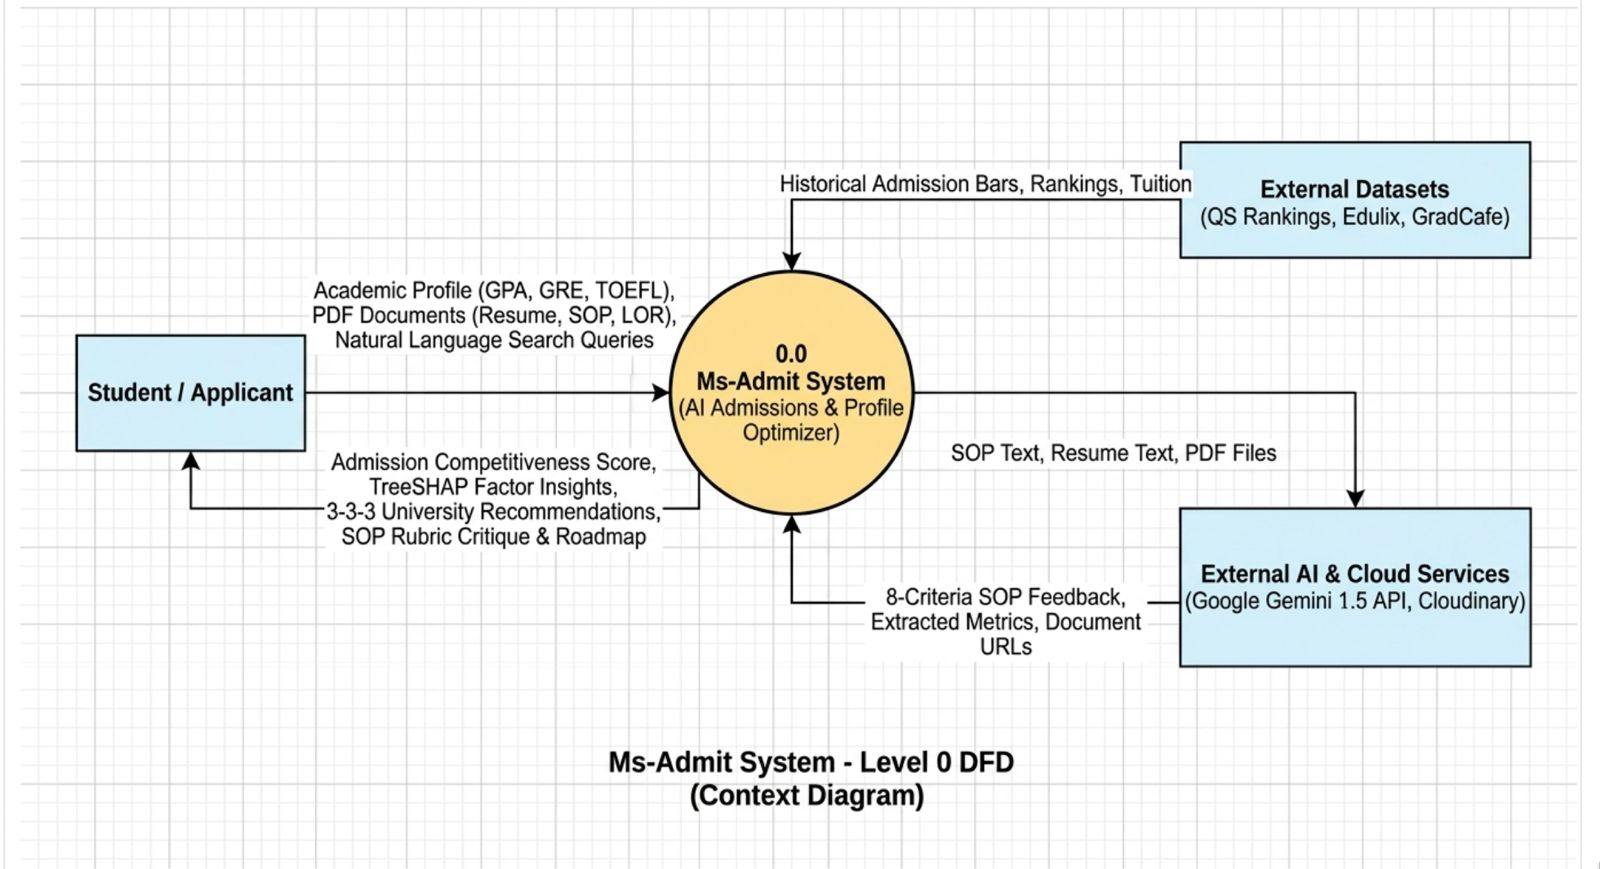
\includegraphics[width=0.85\textwidth]{DFD_0.jpg}
    \caption{DFD Level 0 of MS-Admit}
    \label{fig:dfd_level_0}
\end{figure}
Figure~\ref{fig:dfd_level_0} illustrates the Level 0 Data Flow Diagram (DFD) of MsAdmit, presenting the system's interaction with students, external datasets, and AI services. Students provide their academic profiles, test scores, resumes, SOPs, and search queries as input. The system processes this information using admission prediction models and external AI services to generate competitiveness scores, university recommendations, SOP feedback, and personalized improvement roadmaps. External datasets provide information on university rankings, admission trends, and tuition fees, helping MsAdmit deliver relevant and data-driven guidance to students.
\begin{figure}[H]
    \centering
    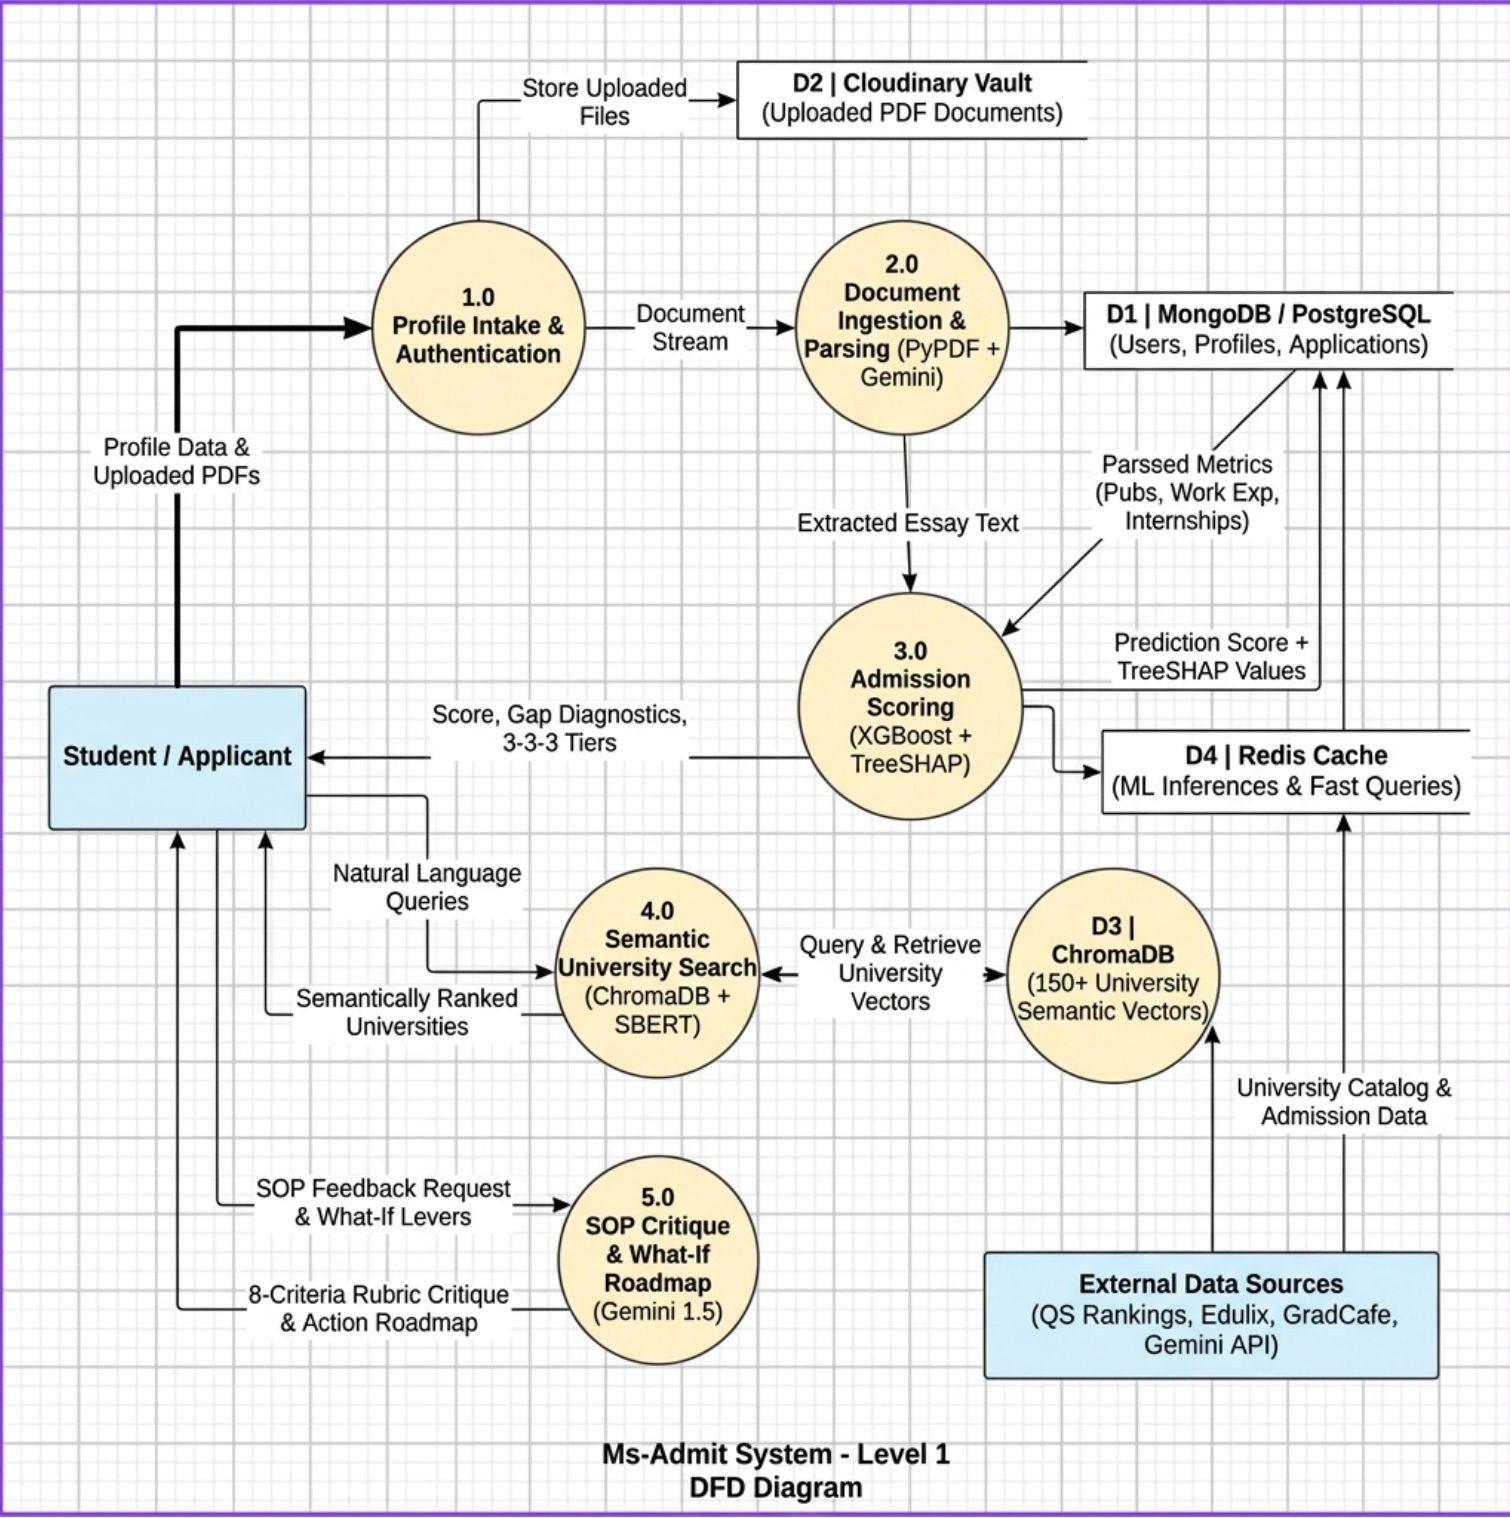
\includegraphics[width=0.85\textwidth]{DFD_1.jpg}
    \caption{DFD Level 1 of MS-Admit}
    \label{fig:dfd_level_1}
\end{figure}
Figure~\ref{fig:dfd_level_1} illustrates the Level 1 Data Flow Diagram (DFD) of MsAdmit, providing a detailed view of its internal processes. The system consists of profile intake and authentication, document ingestion and parsing, admission scoring, semantic university search, and SOP evaluation with a what-if roadmap. These processes interact with databases, caching services, and external data sources to extract relevant information, predict admission competitiveness, recommend suitable universities, and provide personalized feedback to students.
\subsubsection{Cost Analysis}

The operational costs of cloud infrastructure, database services, and external APIs were taken into account while evaluating MsAdmit's economic viability. In order to reduce operational costs while preserving performance and scalability, the system combines premium cloud resources with free-tier services.


%------------------------------------------------
% Estimated Monthly Operational Cost
%------------------------------------------------

\begin{table}[H]
\centering
\caption{Estimated Monthly Operational Cost of MsAdmit}
\label{tab:cost_analysis}
\renewcommand{\arraystretch}{1.3}

\begin{tabularx}{\columnwidth}{|p{2.1cm}|p{2.1cm}|X|p{1.6cm}|}
\hline
\textbf{Service Component} &
\textbf{Provider / Tier} &
\textbf{Operational Purpose} &
\textbf{Monthly Cost} \\
\hline
API Backend Compute &
AWS EC2 t3.medium / Render &
Hosts the FastAPI backend, PDF parsing, and ML inference. &
INR 1,430--2,380 \\
\hline
Frontend Hosting &
Vercel / Netlify &
Hosts and distributes the React frontend. &
INR 0 (Free Tier) \\
\hline
Database &
MongoDB Atlas &
Stores user profiles, prediction results, and application data. &
Depends on usage / free tier \\
\hline
Vector Database &
ChromaDB &
Stores university embeddings for semantic search. &
Included in backend hosting \\
\hline
Caching Service &
Redis Cloud / In-memory Cache &
Improves response time for repeated requests. &
INR 0--950 (estimated) \\
\hline
External LLM API &
Google Gemini 1.5 &
Evaluates SOPs and generates feedback. &
Depends on API usage \\
\hline
Document Storage &
Cloudinary &
Stores uploaded resumes and related documents. &
Depends on usage / free tier \\
\hline
\end{tabularx}
\end{table}

\noindent
 Table 4.1 shows the  estimated monthly
operational costs of MsAdmit and supports its financial feasibility.
The use of free-tier services and scalable infrastructure helps
minimize initial expenses, making the system practical to implement
and maintain. Although costs may increase with user activity and
AI API usage, selecting suitable service plans and optimizing
resource utilization can help ensure the platform remains
cost-effective and sustainable in the long term.


% --- document ---


\clearpage
\subsubsection{Hardware and software requirements}



\begin{table}[H]
\centering
\caption{Hardware Requirements for MsAdmit}
\label{tab:hardware_requirements}

\large
\renewcommand{\arraystretch}{1.8}
\setlength{\tabcolsep}{8pt}

\begin{tabularx}{\textwidth}{
|>{\raggedright\arraybackslash}p{3.2cm}
|>{\raggedright\arraybackslash}p{3.2cm}
|>{\raggedright\arraybackslash}p{3.2cm}
|X|}
\hline
\textbf{Component} &
\textbf{Minimum Requirement} &
\textbf{Recommended Requirement} &
\textbf{Purpose} \\
\hline

Processor &
Intel Core i3 or equivalent &
Intel Core i5 or equivalent &
Runs the application and development tools. \\
\hline

RAM &
8 GB &
16 GB or more &
Supports backend services, database operations, and development tools. \\
\hline

Storage &
10 GB free space &
20 GB or more free space &
Stores source code, dependencies, datasets, and project files. \\
\hline

Internet Connection &
Stable broadband connection &
High-speed broadband connection &
Enables API access, cloud services, and university data retrieval. \\
\hline
\end{tabularx}
\end{table}

\justify
The Table 4.2 shows hardware requirements for MsAdmit includes a suitable processor, sufficient RAM, adequate storage, a display, and a stable internet connection. These resources support application development, database operations, machine learning tasks, and access to external AI services. The recommended specifications help ensure smooth execution of the system and efficient performance during development and testing.


\begin{table}[H]
\centering
\caption{Software Requirements for MsAdmit}
\label{tab:software_requirements}
\renewcommand{\arraystretch}{1.3}
\begin{tabularx}{\textwidth}{
|>{\raggedright\arraybackslash}p{3cm}
|>{\raggedright\arraybackslash}p{3cm}
|>{\raggedright\arraybackslash}p{3cm}
|X|}
\hline
\textbf{Software / Technology} &
\textbf{Version / Platform} &
\textbf{Category} &
\textbf{Purpose} \\
\hline
Python &
3.10 or compatible &
Programming Language &
Implements the backend, data processing, and machine learning components. \\
\hline
FastAPI &
Compatible version &
Backend Framework &
Provides APIs for profile evaluation and system functionality. \\
\hline
Next.js &
Compatible version &
Frontend Framework &
Develops the user interface and interactive application pages. \\
\hline
MongoDB Atlas &
Cloud-based &
Database &
Stores user profiles, prediction results, and application information. \\
\hline
XGBoost &
Compatible version &
Machine Learning &
Predicts admission competitiveness using applicant profile data. \\
\hline
SHAP &
Compatible version &
Explainable AI &
Explains the factors influencing model predictions. \\
\hline
ChromaDB &
Compatible version &
Vector Database &
Supports semantic search using university data embeddings. \\
\hline
Redis &
Compatible version &
Caching &
Improves response times by caching frequently accessed data. \\
\hline
Google Gemini API &
API-based service &
Generative AI &
Supports SOP evaluation and feedback generation. \\
\hline
Visual Studio Code &
Compatible version &
Development Environment &
Provides an environment for writing and debugging code. \\
\hline
Git and GitHub &
Web-based / compatible version &
Version Control &
Tracks code changes and supports collaborative development. \\
\hline
Web Browser &
Chrome, Firefox, or Safari &
Application Access &
Allows users to access the MsAdmit web application. \\
\hline
\end{tabularx}
\end{table}
\justify
The Table 4.3 shows software requirements for MsAdmit includes the technologies needed to develop and operate the system. Python, FastAPI, and Next.js support backend and frontend development, while MongoDB manages data storage. XGBoost and SHAP enable admission predictions and explainability, and ChromaDB supports semantic university searches. Redis provides caching, while the Gemini API assists with SOP evaluation and feedback generation. Together, these technologies ensure efficient system functionality and personalized admission guidance.

\section{System architecture}



\subsection{UI/UX Diagram}

\begin{figure}[!htbp]
    \centering
    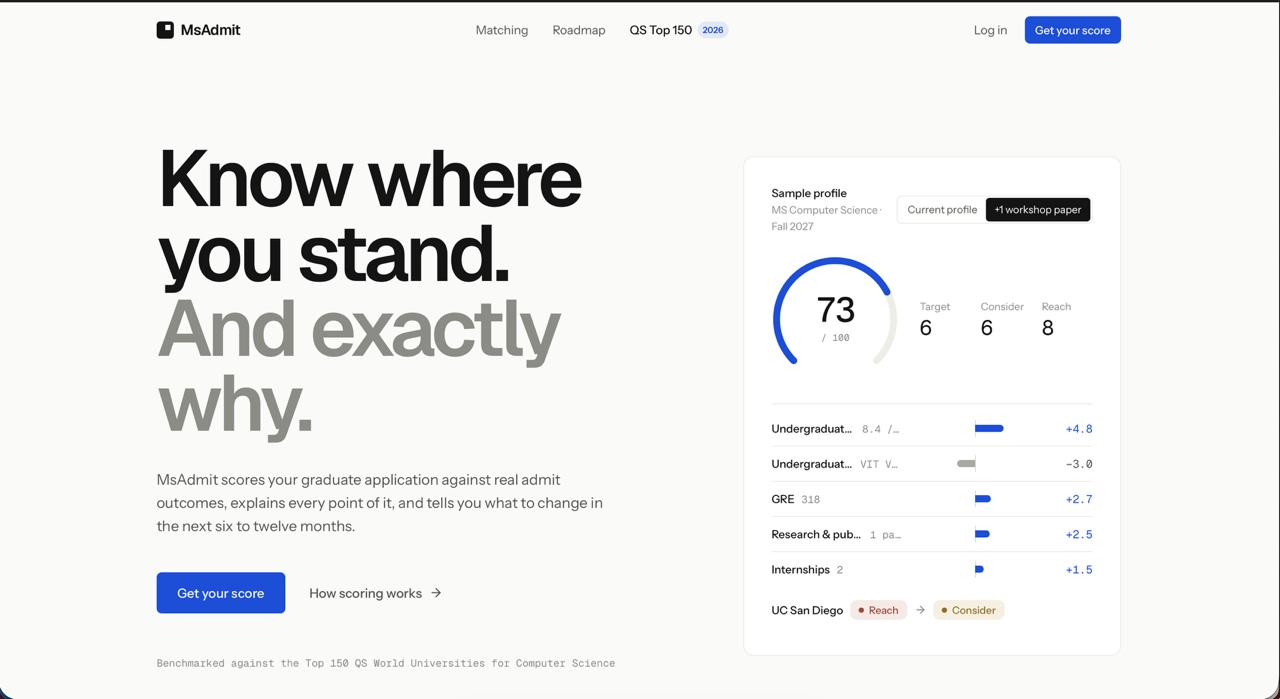
\includegraphics[width=0.85\textwidth]{uiux.jpeg}
    \caption{UI/UX Diagram of MsAdmit}
    \label{fig:uiux}
\end{figure}

\noindent
Figure \ref{fig:uiux} illustrates the homepage of MsAdmit, 
featuring a clean interface, university matching, personalized 
improvement roadmaps, and university rankings. The dashboard 
displays the admission competitiveness score and factors 
influencing the student's profile.



\subsection{Block Diagram}

\begin{figure}[!htbp]
    \centering
    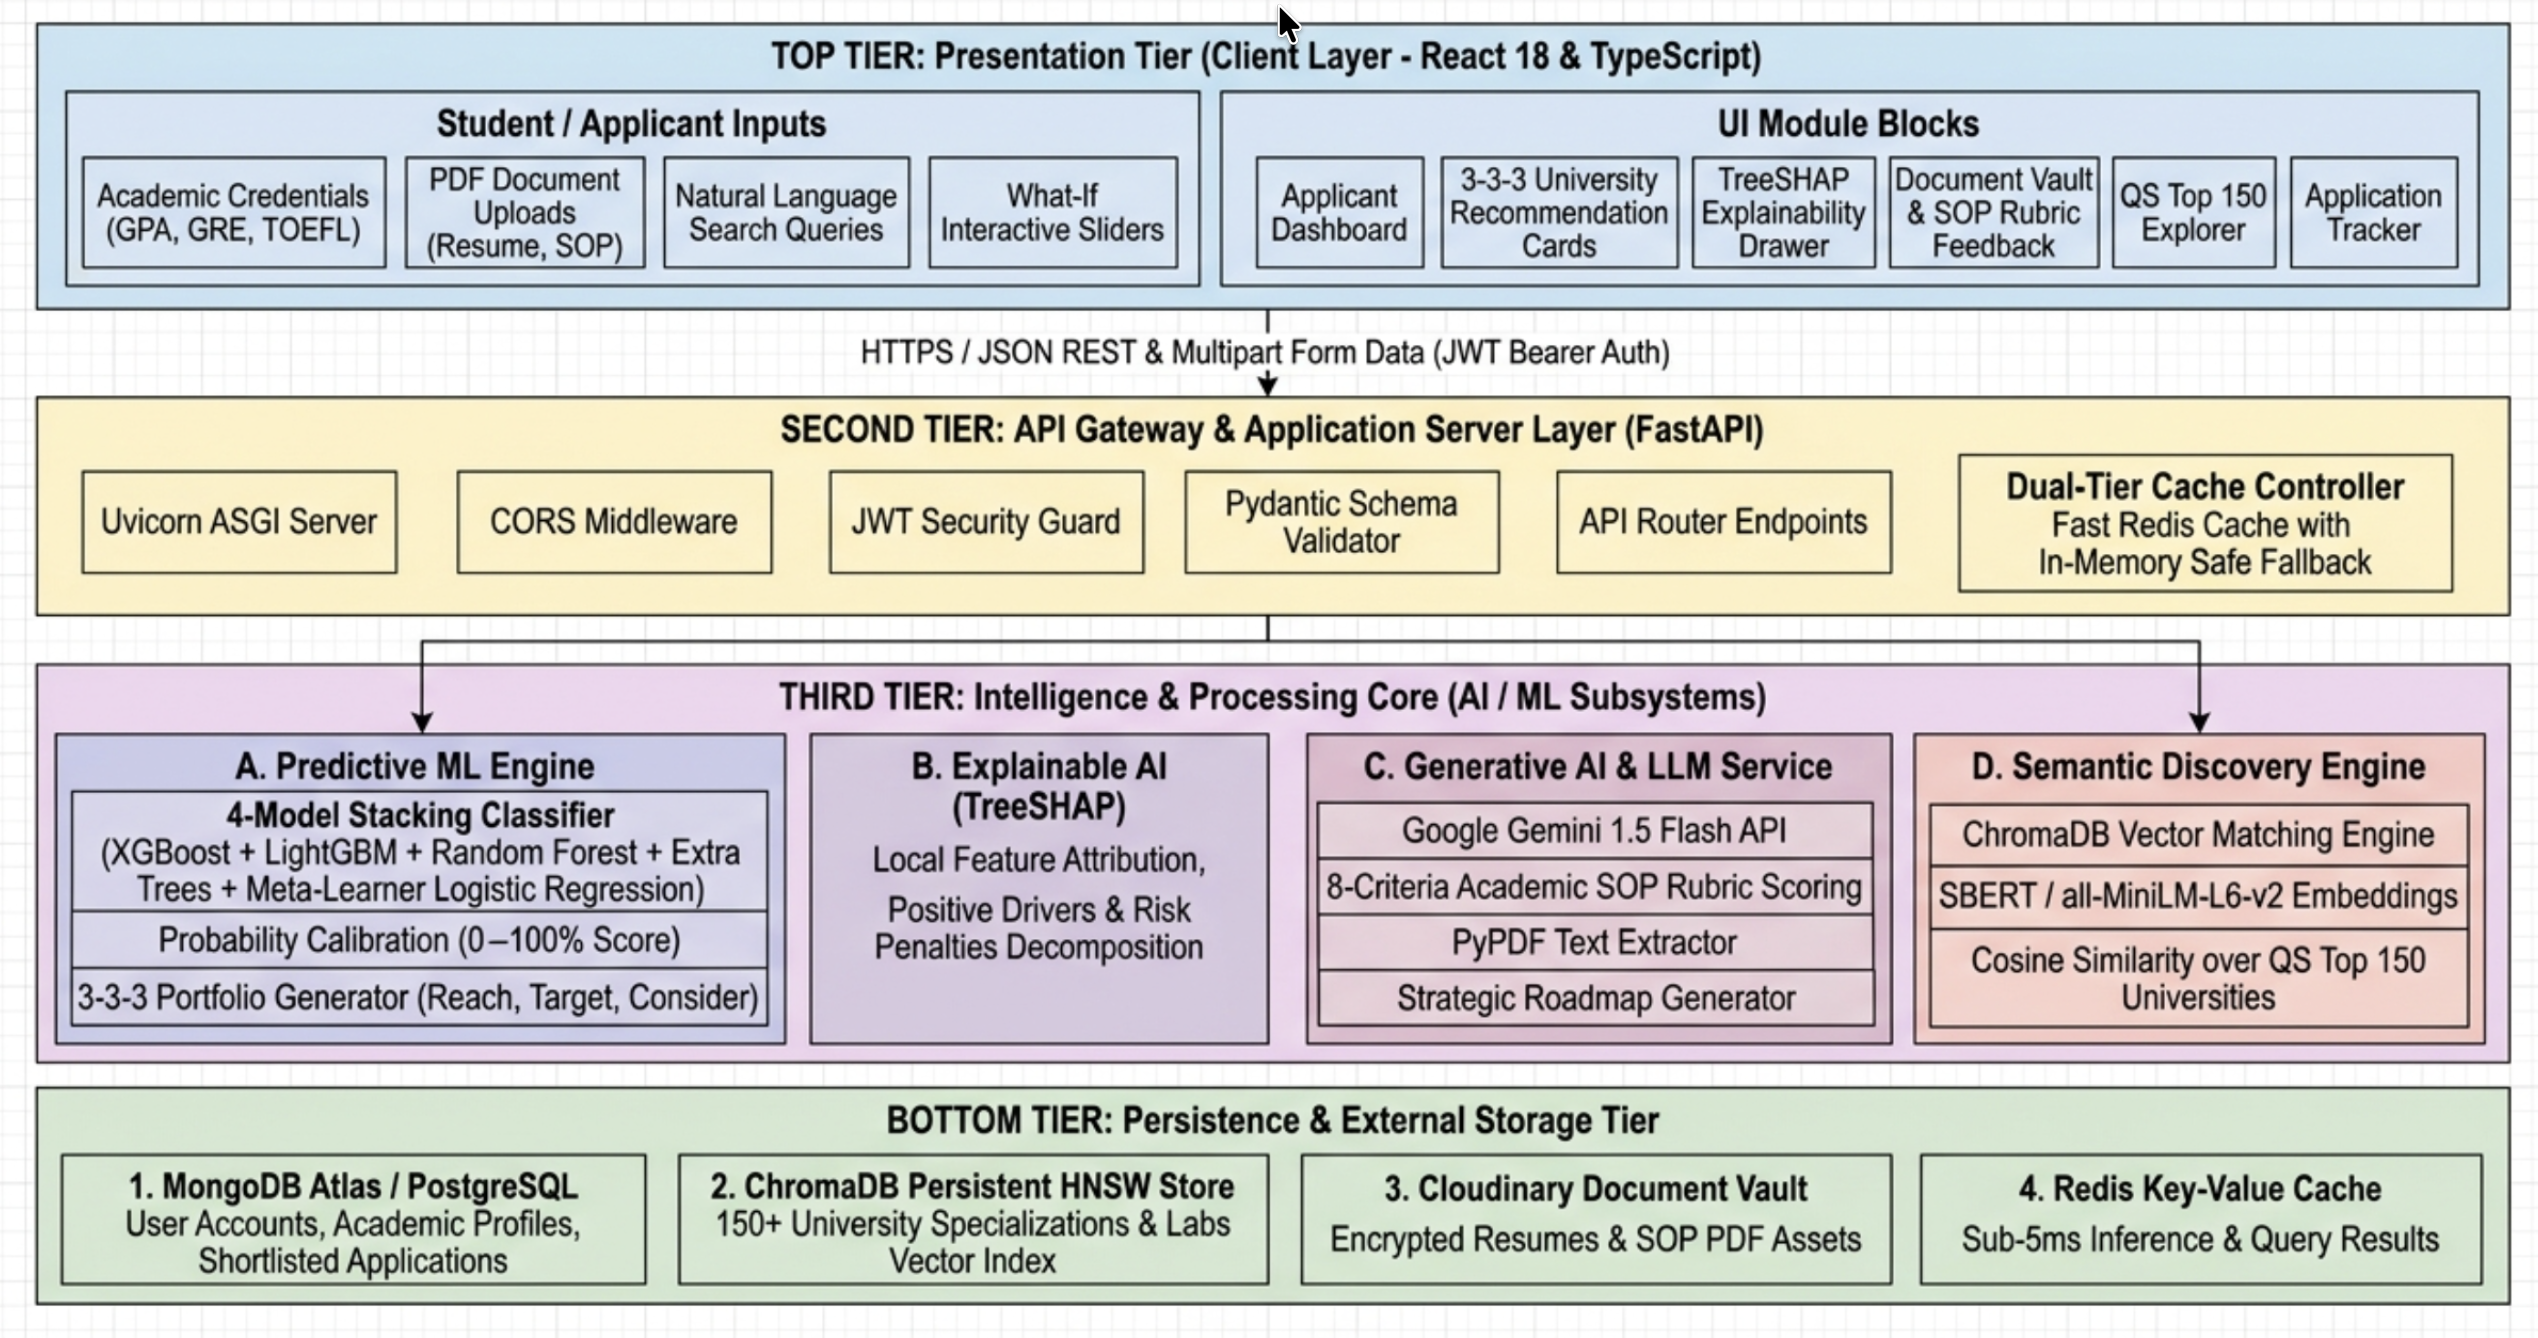
\includegraphics[width=0.95\textwidth]{Screenshot 2026-10-27 at 3.10.37 PM.png}
    \caption{Block Diagram of MsAdmit}
    \label{fig:blockdiagram}
\end{figure}

\newpage
\justify
Figure \ref{fig:blockdiagram}illustrates the overall system architecture of MsAdmit, showing the interaction between the presentation layer, API gateway, AI/ML processing core, and persistence and external storage layer. These components work together to predict admission probabilities, explain model predictions, evaluate Statements of Purpose (SOPs), recommend suitable universities, and manage applicant profiles and application data.


\justify
This chapter presented the system design of MsAdmit, covering requirement engineering, the software development lifecycle, functional and non-functional requirements, cost analysis, and hardware and software requirements. It also described the system architecture, data flow diagrams, and UI/UX design, explaining how the different components work together to provide admission prediction, university recommendations, SOP evaluation, and personalized guidance.



\chapter{Result and Discussion} \label{chap5}
\newpage
\justify
This section presents the implemented interfaces and key functionalities of the MsAdmit system through screenshots captured from the application. Each figure illustrates a specific feature, including student profile intake and resume extraction, applicant dashboard, AI-based university recommendations, semantic university search, SOP evaluation, what-if simulation, and application tracking. Brief descriptions accompany each screenshot to explain its purpose and demonstrate how the system supports students throughout the graduate admission process.
\section{Screenshots of the System}

The visual interfaces and functional screens of the MsAdmit system are presented below with academic figure captions and descriptive explanations.

% Figure 5.1
\begin{figure}[!htbp]
    \centering
    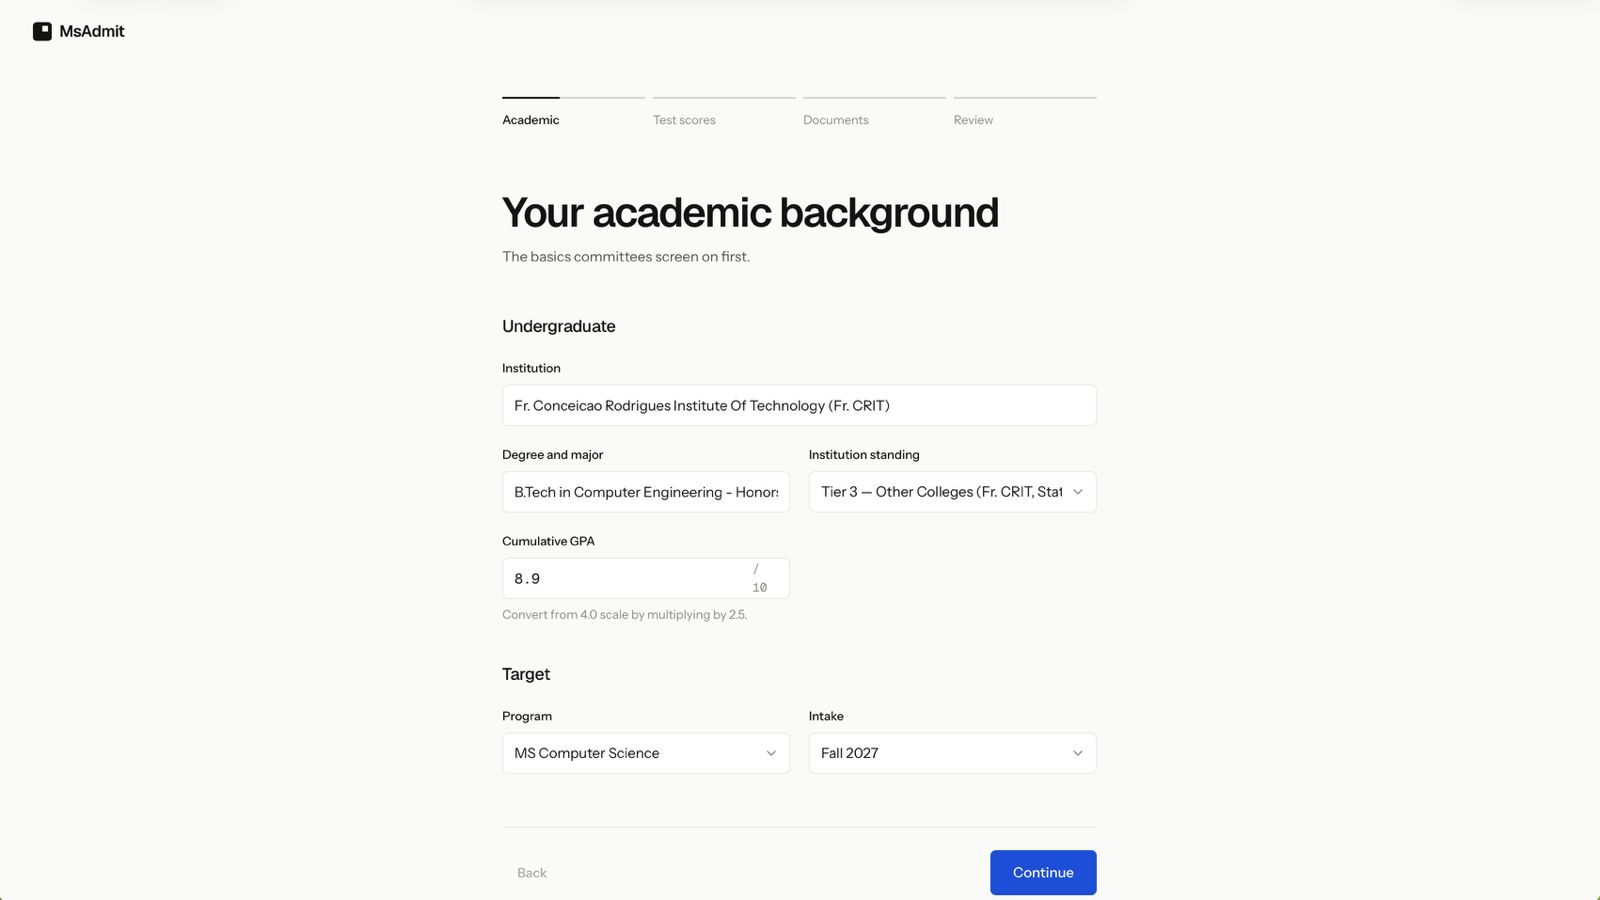
\includegraphics[width=0.85\textwidth]{figure5_1.png}
    \caption{Student Profile Intake \& Resume Extraction Interface}
    \label{fig:profile-intake}

    \vspace{0.2cm}
    \begin{minipage}{0.9\textwidth}
        \small
        Figure~\ref{fig:profile-intake} Displays the initial profile intake interface where applicants can either manually enter academic metrics or upload a PDF resume. The backend extracts relevant work experience (in months), internships, and research papers, automatically populating the form.
    \end{minipage}
\end{figure}

% Figure 5.2
\begin{figure}[!htbp]
    \centering
    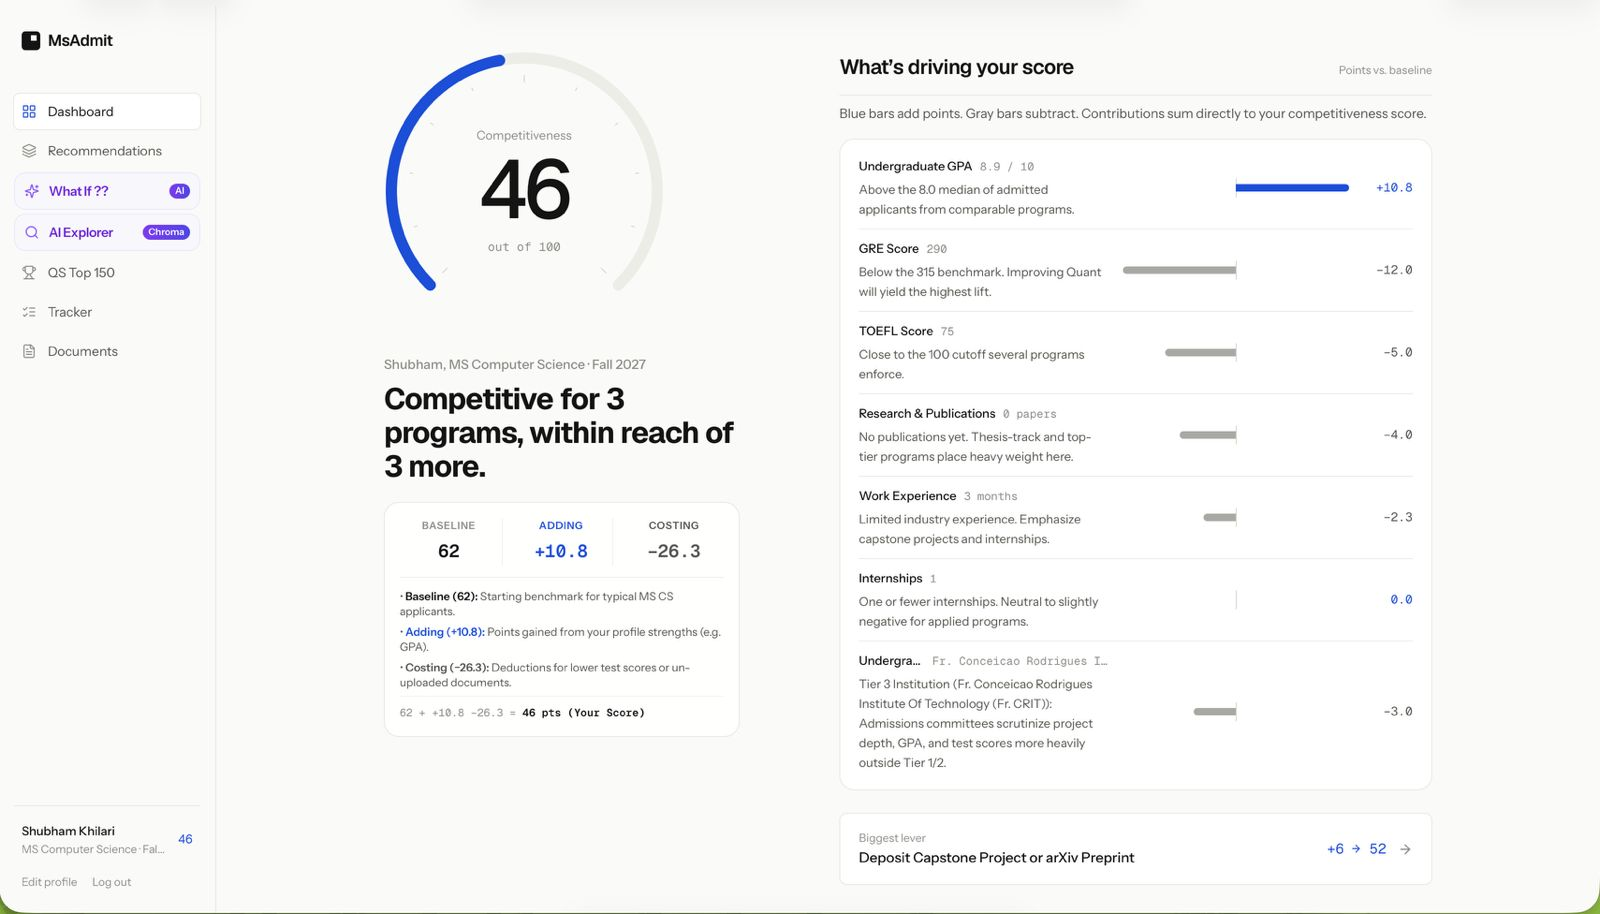
\includegraphics[width=0.85\textwidth]{figure5_2.png}
    \caption{Comprehensive Applicant Dashboard }
    \label{fig:applicant-dashboard}

    \vspace{0.2cm}
    \begin{minipage}{0.9\textwidth}
        \small
        Figure~\ref{fig:applicant-dashboard} Shows the centralized applicant dashboard displaying the calibrated overall Competitiveness Score (0\%--100\%), an alert for the closest upcoming application deadline, an interactive quick-action panel, and a summary breakdown of 3-3-3 university tiers.
    \end{minipage}
\end{figure}

% Figure 5.3
\begin{figure}[!htbp]
    \centering
    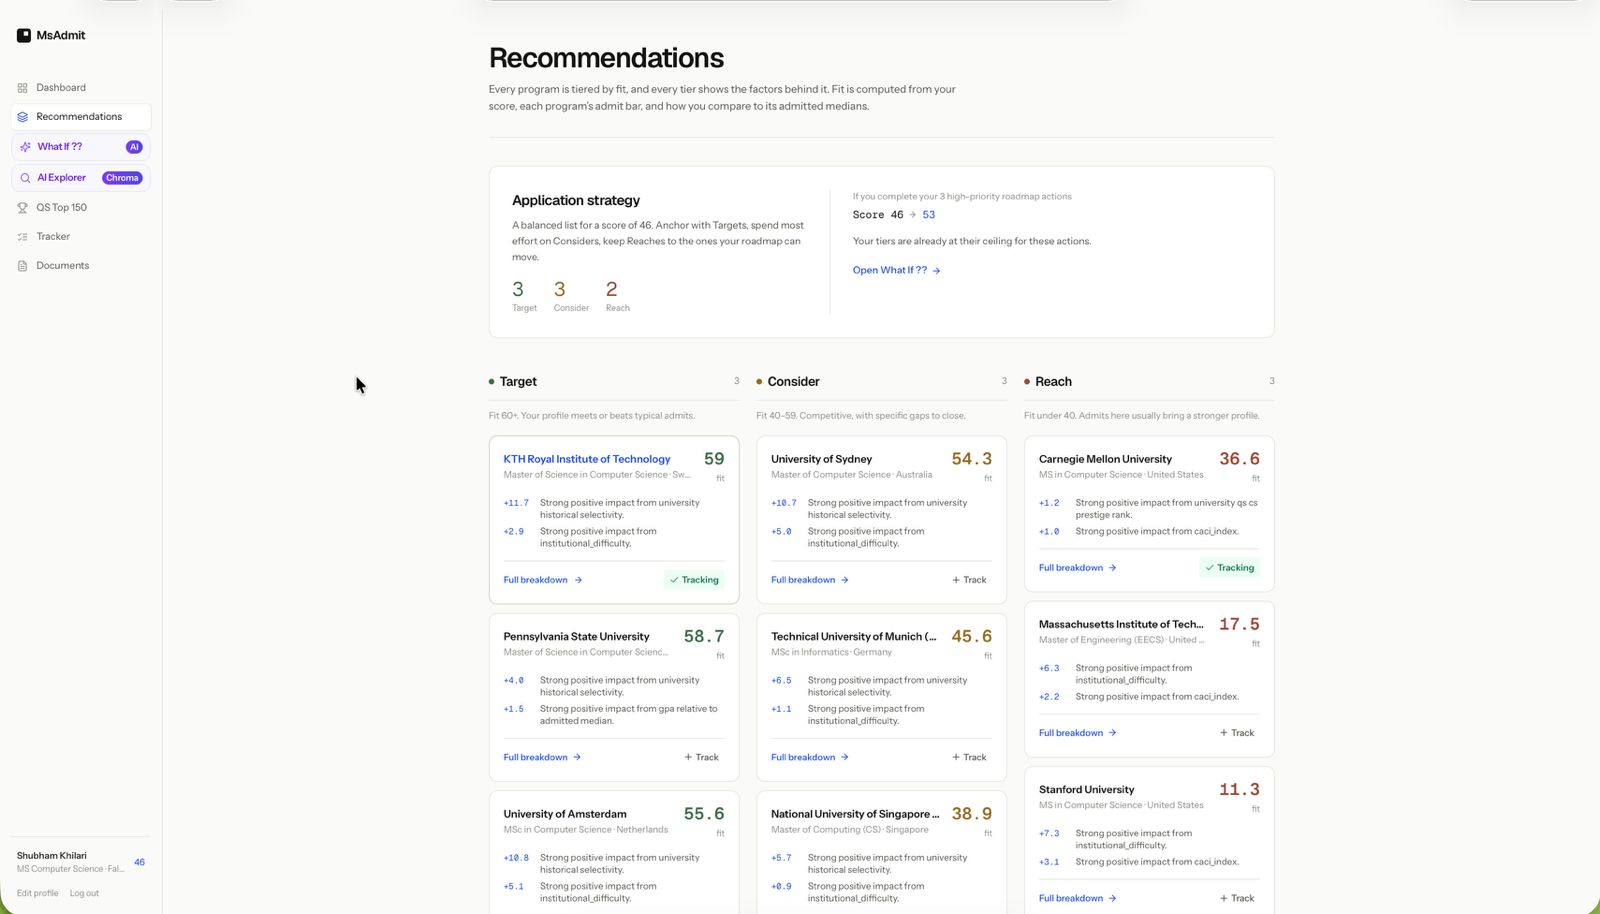
\includegraphics[width=0.85\textwidth]{figure5_3.png}
    \caption{AI University Recommendations with TreeSHAP Explainability Drawer}
    \label{fig:university-recommendations}

    \vspace{0.2cm}
    \begin{minipage}{0.9\textwidth}
        \small
        Figure~\ref{fig:university-recommendations} Demonstrates the recommendation interface displaying categorized Reach, Target, and Consider institution cards. Clicking any university expands the TreeSHAP slide-out drawer, illustrating positive drivers such as strong GPA and publications, along with risk factors such as lower GRE scores or missing work experience.
    \end{minipage}
\end{figure}

% Figure 5.4
\begin{figure}[!htbp]
    \centering
    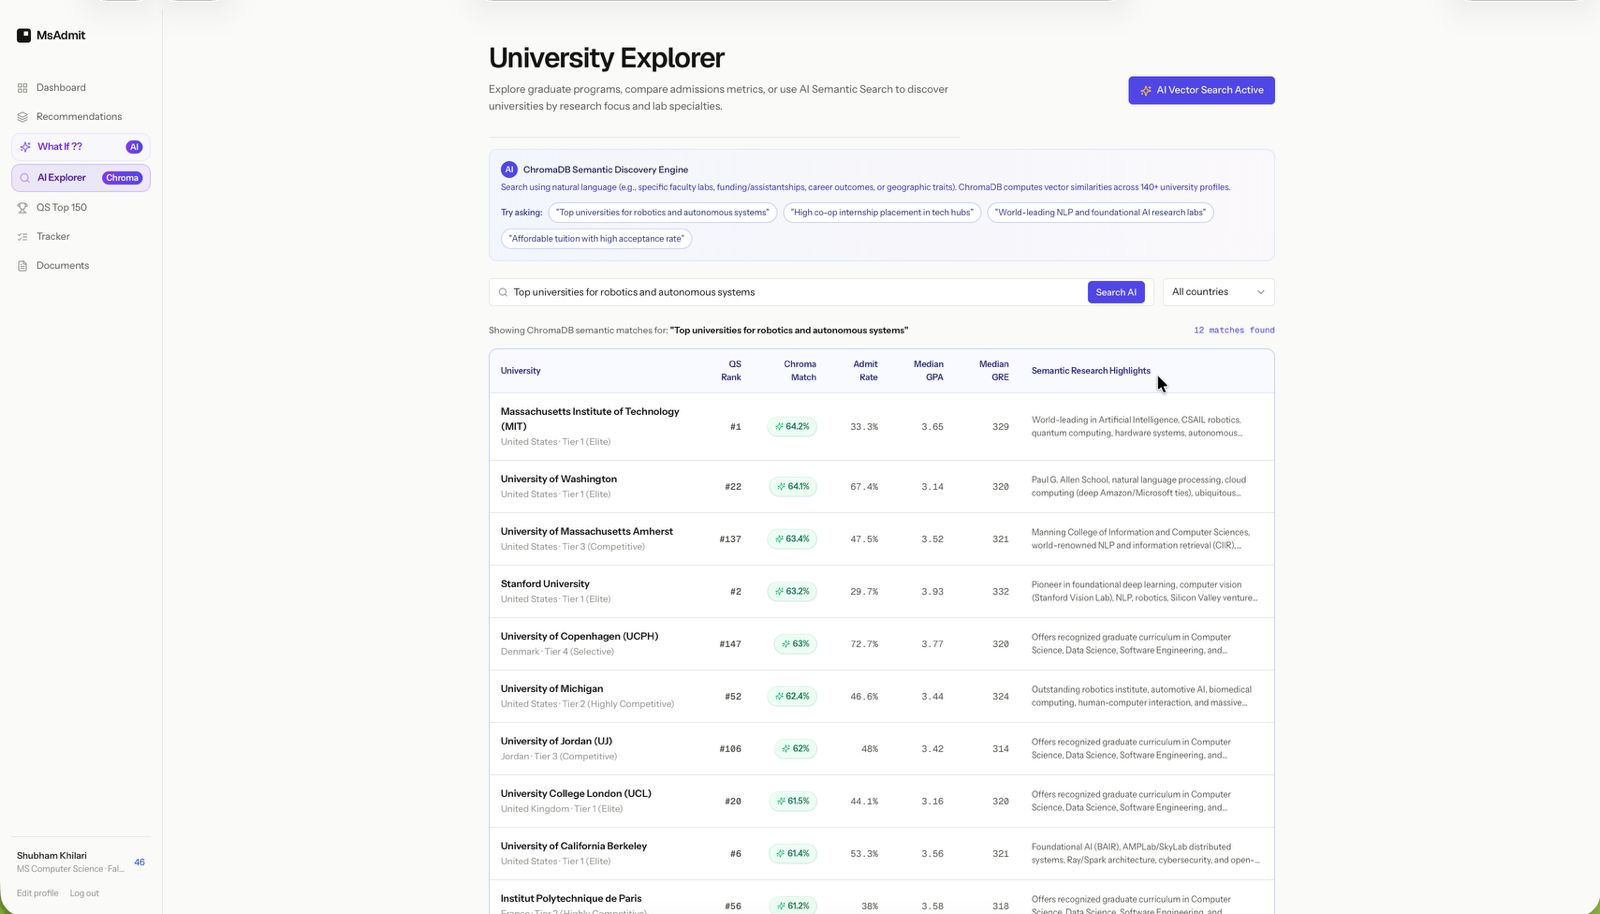
\includegraphics[width=0.85\textwidth]{figure5_4.png}
    \caption{Semantic University Explorer \& Top 150 Rankings Table}
    \label{fig:university-explorer}

    \vspace{0.2cm}
    \begin{minipage}{0.9\textwidth}
        \small
        Figure~\ref{fig:university-explorer} Displays the natural-language semantic search bar powered by ChromaDB. Students can search for research programs, such as AI and robotics with affordable tuition, and explore matching institutions alongside their median admission requirements.
    \end{minipage}
\end{figure}

% Figure 5.5
\begin{figure}[!htbp]
    \centering
    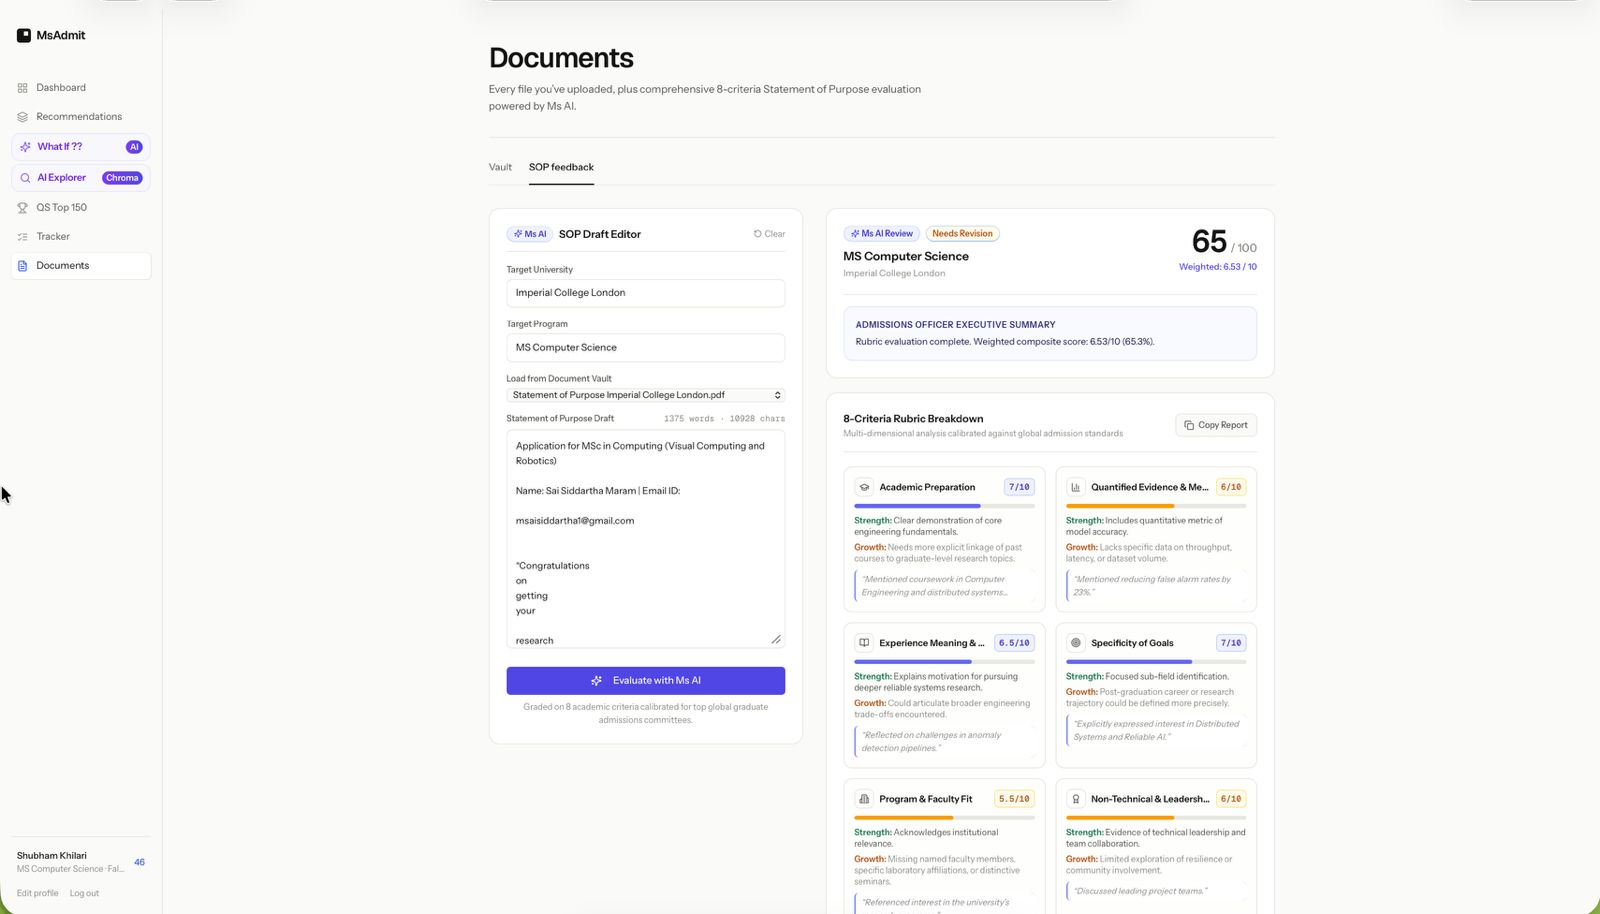
\includegraphics[width=0.85\textwidth]{figure5_5.png}
    \caption{Document Vault \& Gemini 1.5 8-Criteria SOP Evaluation Interface}
    \label{fig:document-vault}

    \vspace{0.2cm}
    \begin{minipage}{0.9\textwidth}
        \small
        Figure~\ref{fig:document-vault} Displays the document evaluation workspace showing an uploaded Statement of Purpose, a radar or progress breakdown across the eight criteria, and paragraph-by-paragraph revision suggestions.
    \end{minipage}
\end{figure}

% Figure 5.6
\begin{figure}[!htbp]
    \centering
    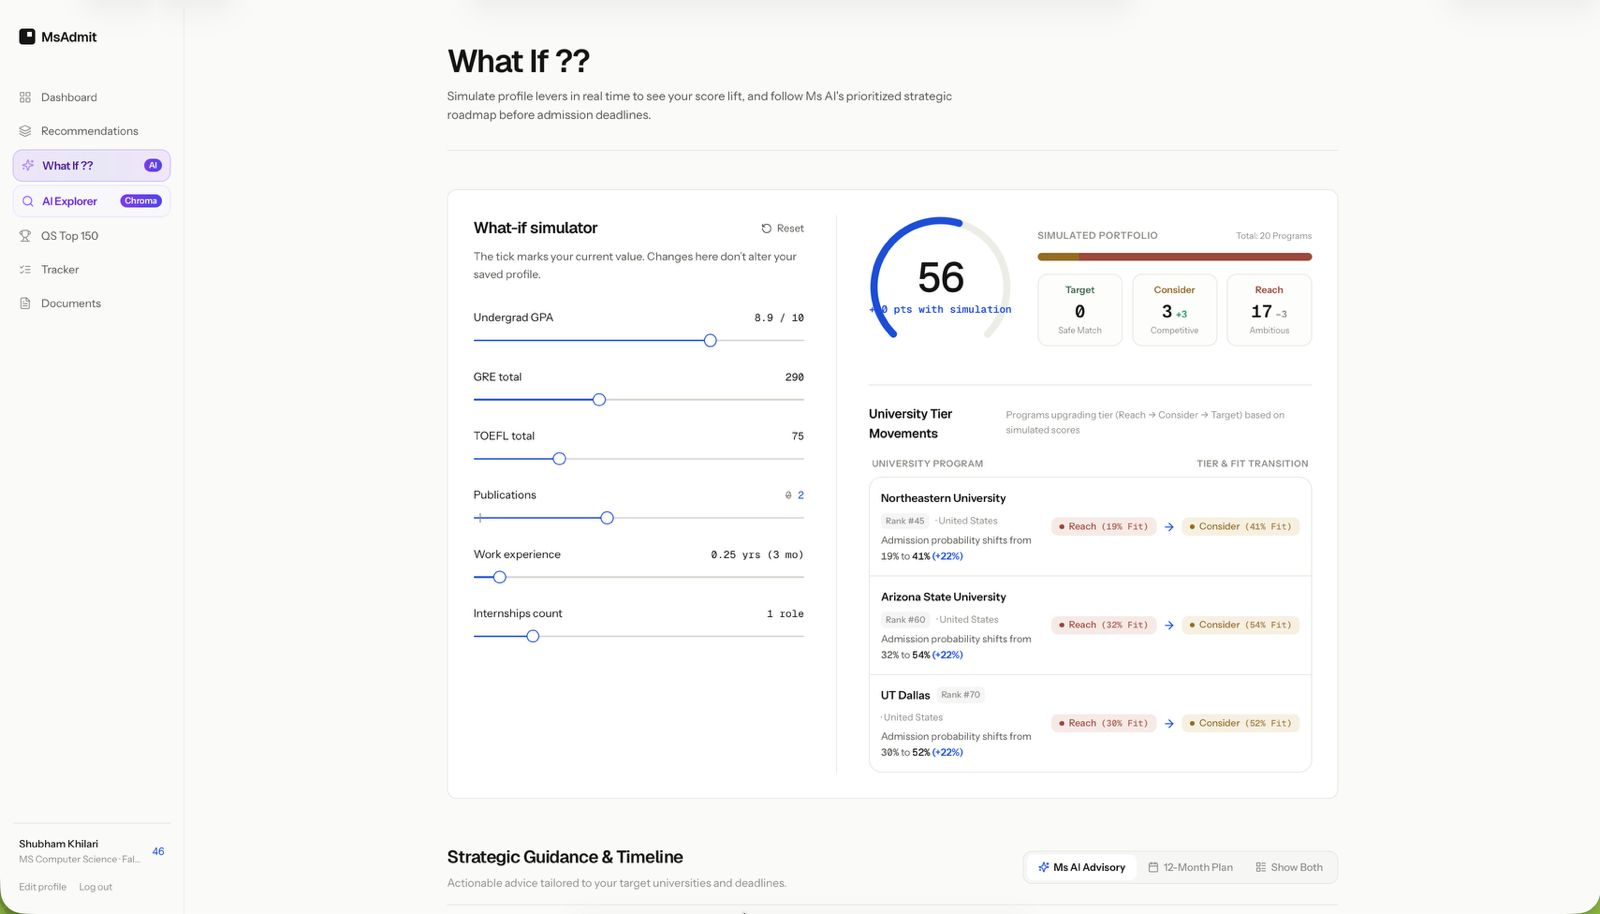
\includegraphics[width=0.85\textwidth]{figure5_6.png}
    \caption{Interactive What-If Simulator \& Dynamic Optimization Roadmap}
    \label{fig:optimization-roadmap}

    \vspace{0.2cm}
    \begin{minipage}{0.9\textwidth}
        \small
        Figure~\ref{fig:optimization-roadmap} Illustrates the What-If simulation workspace where students can adjust GRE Quantitative and Verbal scores, GPA, and research publications to observe real-time recalculations of admission probabilities and updated university tier classifications.
    \end{minipage}
\end{figure}

% Figure 5.7
\begin{figure}[!htbp]
    \centering
    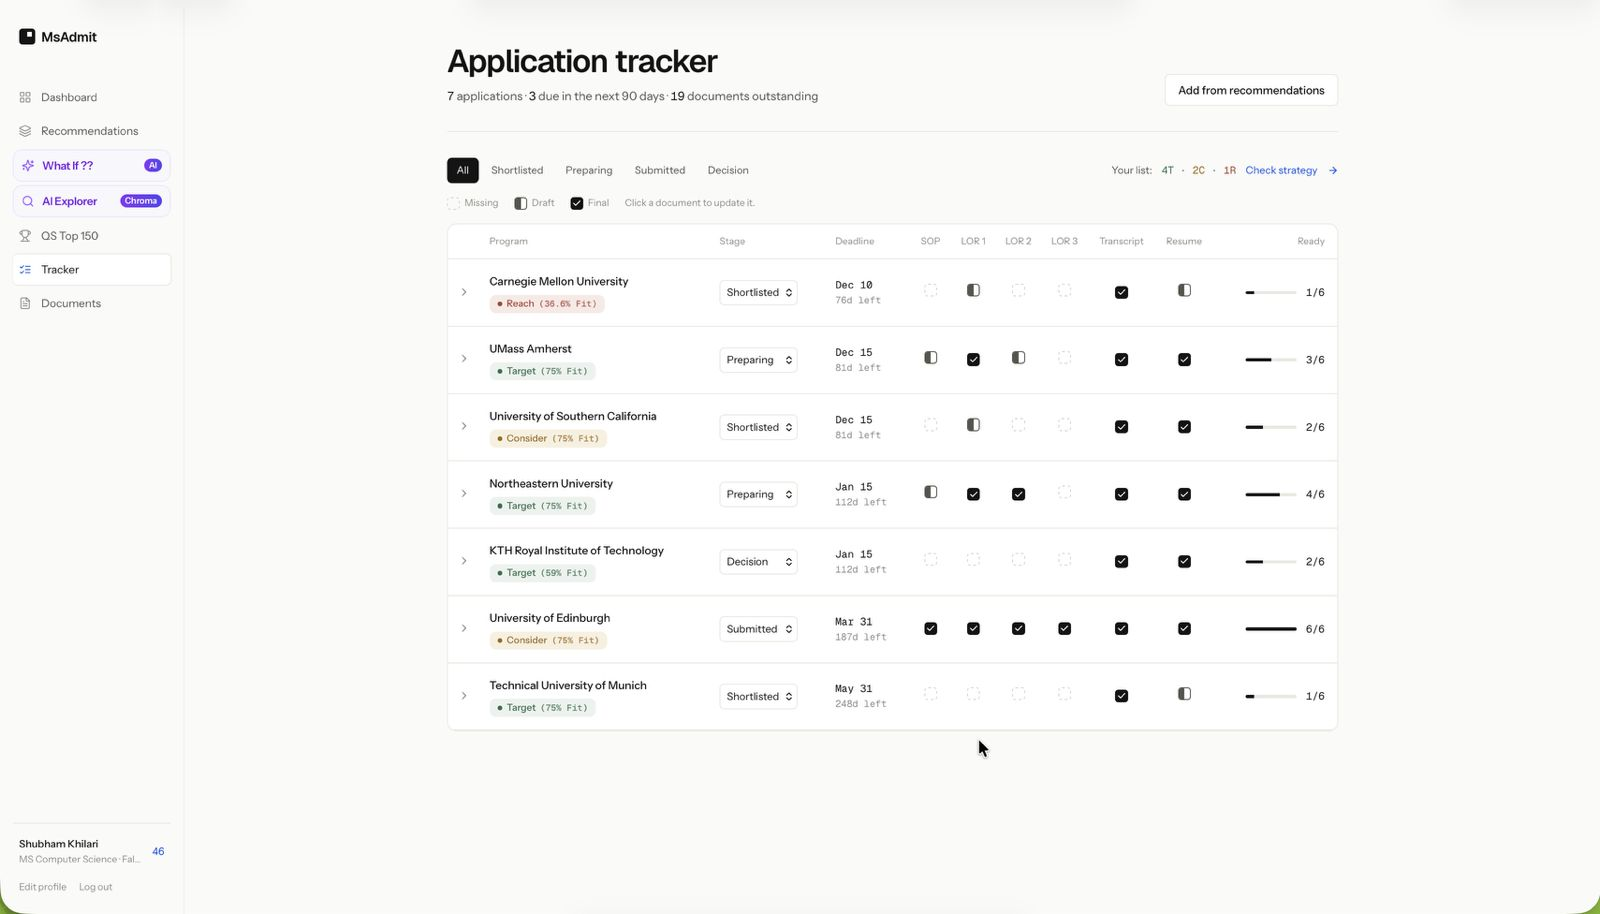
\includegraphics[width=0.85\textwidth]{figure5_7.png}
    \caption{Active Application Tracker \& Document Progress Workspace}
    \label{fig:application-tracker}

    \vspace{0.2cm}
    \begin{minipage}{0.9\textwidth}
        \small
        Figure~\ref{fig:application-tracker} Highlights the application management tracker showing shortlisted programs, a six-stage document checklist (SOP, LOR 1--3, transcripts, and resume), a deadline countdown, and a cumulative application fee budget calculator.
    \end{minipage}
\end{figure}

\clearpage


\section{Sample Code (Key Algorithms \& Core Logic)}

%--------------------------------------------------
% Listing 5.1
%--------------------------------------------------
\subsection{Multi-Model Stacking Ensemble Training and Calibration}

\begin{lstlisting}[language=Python]
from lightgbm import LGBMClassifier
from xgboost import XGBClassifier
from sklearn.ensemble import (
    ExtraTreesClassifier,
    RandomForestClassifier,
    StackingClassifier
)
from sklearn.linear_model import LogisticRegression

def build_stacking_ensemble(X_train, y_train):
    estimators = [
        ('xgb', XGBClassifier(
            n_estimators=300,
            learning_rate=0.025,
            max_depth=6,
            subsample=0.85,
            colsample_bytree=0.85,
            random_state=42
        )),
        ('lgbm', LGBMClassifier(
            n_estimators=300,
            learning_rate=0.03,
            max_depth=6,
            num_leaves=15,
            random_state=42
        )),
        ('rf', RandomForestClassifier(
            n_estimators=150,
            max_depth=14,
            min_samples_leaf=3,
            random_state=42
        )),
        ('et', ExtraTreesClassifier(
            n_estimators=150,
            max_depth=14,
            min_samples_leaf=3,
            random_state=42
        ))
    ]

    stacking_classifier = StackingClassifier(
        estimators=estimators,
        final_estimator=LogisticRegression(
            C=1.0,
            max_iter=500,
            random_state=42
        ),
        cv=5,
        n_jobs=-1,
        passthrough=False
    )

    stacking_classifier.fit(X_train, y_train)
    return stacking_classifier
\end{lstlisting}
This code builds and trains a stacking ensemble classifier that combines XGBoost, LightGBM, Random Forest, and Extra Trees, using Logistic Regression as the meta-classifier to predict admission outcomes.


%--------------------------------------------------
% Listing 5.2
%--------------------------------------------------
\clearpage
\subsection{Admission Prediction and TreeSHAP Attribution Logic}

\begin{lstlisting}[language=Python]
from typing import Dict, Any

def compute_prediction_and_shap(
    profile_input: Dict[str, Any]
) -> Dict[str, Any]:
    """Calculate admission score and profile contributions."""

    engine = get_ml_engine()
    normalized = normalize_profile(profile_input)

    portfolio = engine.recommend_portfolio(
        normalized,
        top_k=3,
        include_shap=True
    )

    gpa = normalized["gpa"]
    gre = normalized["gre"]
    pubs = normalized["research_publications"]
    work_months = int(
        profile_input.get("work_months", 0)
    )

    def clamp(v: float, lo: float, hi: float) -> float:
        return max(lo, min(hi, v))

    gpa_contrib = round(
        clamp((gpa - 8.0) * 12.0, -12.0, 12.0), 1
    )
    gre_contrib = round(
        (gre - 315.0) * 0.9, 1
    )
    research_contrib = round(
        min(10.0, pubs * 3.5), 1
    )
    work_contrib = round(
        min(7.0, work_months / 36.0 * 8.0), 1
    )

    return {
        "overall_score": portfolio.get(
            "overall", 72.0
        ),
        "portfolio": portfolio.get("universities", []),
        "gpa_contribution": gpa_contrib,
        "gre_contribution": gre_contrib,
        "research_contribution": research_contrib,
        "work_contribution": work_contrib
    }
\end{lstlisting}
This function calculates an applicant’s overall admission score, recommends the top three universities, and estimates the individual contributions of GPA, GRE, research publications, and work experience to their profile.

%--------------------------------------------------
% Listing 5.3
%--------------------------------------------------
\clearpage
\subsection{Statement of Purpose Evaluation Using Gemini}

\begin{lstlisting}[language=Python]
import json
import google.generativeai as genai

def evaluate_sop_against_rubric(
    sop_text: str,
    target_university: str
):
    """Evaluate an SOP against eight criteria."""

    prompt = f"""
    Evaluate the following Statement of Purpose for
    {target_university}.

    Score the SOP on eight criteria:
    1. Academic motivation
    2. Program fit
    3. Research interests
    4. Relevant experience
    5. Career goals
    6. Specificity
    7. Structure and clarity
    8. Grammar and writing quality

    Return a JSON object containing scores and
    actionable feedback for each criterion.

    Statement of Purpose:
    {sop_text}
    """

    model = genai.GenerativeModel(
        "gemini-1.5-flash"
    )
    response = model.generate_content(prompt)

    result = json.loads(response.text.strip())
    return result
\end{lstlisting}

\vspace{25pt}
This function uses Google Gemini 1.5 Flash to evaluate a Statement of Purpose against eight criteria, returning a JSON object containing scores and actionable feedback for each criterion.



%--------------------------------------------------
% Listing 5.4
%--------------------------------------------------
\clearpage
\subsection{Semantic University Retrieval Using ChromaDB}

\begin{lstlisting}[language=Python]
import chromadb

class ChromaService:
    def __init__(self, persist_directory: str):
        self.client = chromadb.PersistentClient(
            path=persist_directory
        )

        self.collection = self.client.get_or_create_collection(
            name="universities_semantic_catalog",
            metadata={"hnsw:space": "cosine"}
        )

    def search_universities(
        self,
        query_embedding,
        top_k: int = 10
    ):
        results = self.collection.query(
            query_embeddings=[query_embedding],
            n_results=top_k
        )

        matches = []

        distances = results.get("distances", [[]])[0]
        ids = results.get("ids", [[]])[0]
        documents = results.get("documents", [[]])[0]
        metadatas = results.get("metadatas", [[]])[0]

        for i, dist in enumerate(distances):
            matches.append({
                "id": ids[i],
                "document": documents[i],
                "metadata": metadatas[i],
                "similarity": 1.0 - dist
            })

        return matches
\end{lstlisting}

\vspace{25pt}

This code implements a ChromaDB-based semantic search service that retrieves the top matching universities using embedding similarity and returns their IDs, documents, metadata, and similarity scores.


%--------------------------------------------------
% Listing 5.5
%--------------------------------------------------
\clearpage
\subsection{Hybrid In-Memory Cache with TTL Fallback}

\begin{lstlisting}[language=Python]
import time
import threading

class SafeInMemoryCache:
    def __init__(self, default_ttl: int = 300):
        self.store = {}
        self.lock = threading.Lock()
        self.default_ttl = default_ttl

    def get(self, key):
        with self.lock:
            item = self.store.get(key)

            if item is None:
                return None

            value, expiry = item

            if time.time() >= expiry:
                del self.store[key]
                return None

            return value

    def set(self, key, value, ttl=None):
        if ttl is None:
            ttl = self.default_ttl

        expiry = time.time() + ttl

        with self.lock:
            self.store[key] = (value, expiry)

    def delete(self, key):
        with self.lock:
            self.store.pop(key, None)

    def clear(self):
        with self.lock:
            self.store.clear()
\end{lstlisting}
\vspace{25p}
This code implements a thread-safe in-memory cache with TTL (Time To Live) that stores key-value pairs temporarily, automatically removes expired entries, and supports retrieving, setting, deleting, and clearing cached data.

\clearpage

\section{Testing}

A rigorous three-tier verification pyramid comprising
\textbf{Unit Testing, Integration Testing, and Blackbox Testing} was
executed to validate system accuracy, numerical stability, API security,
and fault tolerance.

%==================================================
% 5.3.1 UNIT TESTING -- OWN PAGE
%==================================================

\subsection{Unit Testing}

\begingroup
\small
\setlength{\tabcolsep}{4pt}
\renewcommand{\arraystretch}{1.4}



\begin{table}[htbp]
\centering
\caption{Unit Testing Results for the MsAdmit System}
\label{tab:unit-testing}

\normalsize
\renewcommand{\arraystretch}{1.7}
\setlength{\tabcolsep}{6pt}

\begin{tabularx}{\textwidth}{
|>{\centering\arraybackslash}p{1.0cm}
|>{\raggedright\arraybackslash}X
|>{\raggedright\arraybackslash}X
|>{\raggedright\arraybackslash}X
|>{\raggedright\arraybackslash}X
|>{\centering\arraybackslash}p{1.2cm}|}
\hline
\textbf{Test ID} &
\textbf{Module / Function} &
\textbf{Input Test Data} &
\textbf{Expected Output} &
\textbf{Actual Result} &
\textbf{Status} \\
\hline

UT-01 &
\makecell[l]{\texttt{normalize\_}\\\texttt{profile()}} &
Indian CGPA = 8.8 / 10.0 &
Scaled GPA = 3.52 / 4.0 &
Scaled GPA = 3.52 &
PASS \\
\hline

UT-02 &
\makecell[l]{\texttt{normalize\_}\\\texttt{profile()}} &
Standard US GPA = 3.75 &
Unchanged GPA = 3.75 &
GPA = 3.75 &
PASS \\
\hline

UT-03 &
TreeSHAP Clamping &
Outlier GRE = 340 &
Contribution capped at +12.0\% &
Contribution = +12.0\% &
PASS \\
\hline

UT-04 &
\makecell[l]{\texttt{extract\_text\_}\\\texttt{from\_pdf()}} &
2-page resume PDF &
Extracted string $\geq$ 500 chars &
Extracted 1,420 chars &
PASS \\
\hline

UT-05 &
\makecell[l]{SafeInMemory\\Cache} &
Key set TTL = 1s; read at 1.5s &
Expired, returns None &
Returned None &
PASS \\
\hline

UT-06 &
\makecell[l]{\texttt{CRITERIA\_}\\\texttt{WEIGHTS}} &
Sum of 8 criteria weights &
Exact cumulative sum = 1.00 &
Sum = 1.0000 &
PASS \\
\hline

\end{tabularx}
\end{table}



The Table 5.1 shows  unit testing results demonstrate that all six test cases passed.
The tests verified GPA normalization, TreeSHAP contribution clamping,
PDF text extraction, cache expiration, and SOP evaluation criteria
weight validation. These results indicate that the tested components
performed as expected under the specified test conditions.

\endgroup


%==================================================
% 5.3.2 INTEGRATION TESTING -- OWN PAGE
%==================================================
\clearpage
\subsection{Integration Testing}

\begingroup
\small
\setlength{\tabcolsep}{3pt}
\renewcommand{\arraystretch}{1.35}



\begin{table}[htbp]
\centering
\caption{Integration Testing Results for the MsAdmit System}
\label{tab:integration-testing}

\normalsize
\setlength{\tabcolsep}{5pt}
\renewcommand{\arraystretch}{1.6}

\begin{tabularx}{\textwidth}{
|>{\centering\arraybackslash}p{1.0cm}
|>{\raggedright\arraybackslash}X
|>{\raggedright\arraybackslash}X
|>{\raggedright\arraybackslash}X
|>{\raggedright\arraybackslash}X
|>{\centering\arraybackslash}p{1.2cm}|}
\hline
\textbf{Test ID} &
\textbf{Subsystems Tested} &
\textbf{Execution Flow} &
\textbf{Expected Behavior} &
\textbf{Actual Result} &
\textbf{Status} \\
\hline

IT-01 &
Client $\rightarrow$ API $\rightarrow$ DB &
\texttt{/auth/signup} &
User created, password hashed, JWT returned &
Status 201; JWT verified &
PASS \\
\hline

IT-02 &
Client $\rightarrow$ Predict $\rightarrow$ ML &
\texttt{/predict} &
Ensemble generates 3-3-3 tiers &
Score and 9 universities returned &
PASS \\
\hline

IT-03 &
Router $\rightarrow$ Redis Cache &
Duplicate \texttt{/predict} &
Cached response in $<$10 ms &
Cache hit; latency 4.2 ms &
PASS \\
\hline

IT-04 &
Docs $\rightarrow$ PyPDF $\rightarrow$ Gemini &
\texttt{/documents/evaluate} &
Text extracted; 8 scores returned in JSON &
8 criteria scores and feedback returned &
PASS \\
\hline

IT-05 &
Explorer $\rightarrow$ ChromaDB &
\texttt{/search} &
Matching universities ranked &
6 ranked universities with scores &
PASS \\
\hline

IT-06 &
Tracker $\rightarrow$ MongoDB &
\texttt{PATCH /profile} &
Checklist update persisted &
Application record updated &
PASS \\
\hline

\end{tabularx}
\end{table}

\vspace{25pt}


The Table 5.2 shows All six integration tests passed, validating communication among
the client, API, database, Machine Learning model, Redis cache,
document evaluation module, ChromaDB search subsystem, and
MongoDB application tracker.

\endgroup



%==================================================
% 5.3.3 BLACKBOX TESTING -- OWN PAGE
%==================================================
\clearpage
\subsection{Blackbox Testing}

\begingroup
\small
\setlength{\tabcolsep}{4pt}
\renewcommand{\arraystretch}{1.4}



\begin{table}[htbp]
\centering
\caption{Blackbox Testing Results for the MsAdmit System}
\label{tab:blackbox-testing}

\normalsize
\setlength{\tabcolsep}{5pt}
\renewcommand{\arraystretch}{1.6}

\begin{tabularx}{\textwidth}{
|>{\centering\arraybackslash}p{1.0cm}
|>{\raggedright\arraybackslash}X
|>{\raggedright\arraybackslash}X
|>{\raggedright\arraybackslash}X
|>{\raggedright\arraybackslash}X
|>{\centering\arraybackslash}p{1.2cm}|}
\hline
\textbf{Test ID} &
\textbf{Scenario / Feature} &
\textbf{User Input / Action} &
\textbf{Expected Behavior} &
\textbf{Actual Result} &
\textbf{Status} \\
\hline

BT-01 &
Auth Boundary &
Login with unregistered email &
Display invalid credentials (401) &
Alert displayed; access denied &
PASS \\
\hline

BT-02 &
GRE Boundary &
Enter GRE = 350 ($>$ 340) &
Prevent form submission &
Error: GRE must be 260--340 &
PASS \\
\hline

BT-03 &
GPA Boundary &
Enter GPA = 0.0 &
Highlight invalid input &
Submission blocked; GPA must be $>$ 0 &
PASS \\
\hline

BT-04 &
Invalid File Format &
Upload .exe or .png as SOP &
Reject non-PDF files &
File rejected immediately &
PASS \\
\hline

BT-05 &
Empty PDF SOP &
Upload blank PDF &
Notify user of unreadable text &
Warning displayed; no crash &
PASS \\
\hline

BT-06 &
What-If Simulator &
Move GRE slider from 310 to 325 &
Recalculate score and tier &
Probability changes by +8.5\%; tiers updated &
PASS \\
\hline

BT-07 &
Session Expiry &
Open dashboard with expired JWT &
Clear token and redirect to login &
Redirects to login screen &
PASS \\
\hline

\end{tabularx}
\end{table}
\vspace{25pt}

The Table 5.3 shows All seven blackbox tests passed, validating authentication,
input boundary checks, file-upload validation, empty-document
handling, real-time profile simulation, and session-expiry
management. The results indicate that the tested features
responded as expected to the specified user inputs.

\endgroup

\clearpage

\newpage


\subsection{Machine Learning Architecture \& Predictive Modeling Pipeline}

A two-tier stacking ensemble is designed using
\texttt{StackingClassifier}. The base learners (Level 0)
generate out-of-fold probabilistic predictions using
five-fold cross-validation (CV = 5). These predictions are
then passed to a Level-1 Logistic Regression meta-classifier.

\begin{figure}[!htbp]
    \centering
    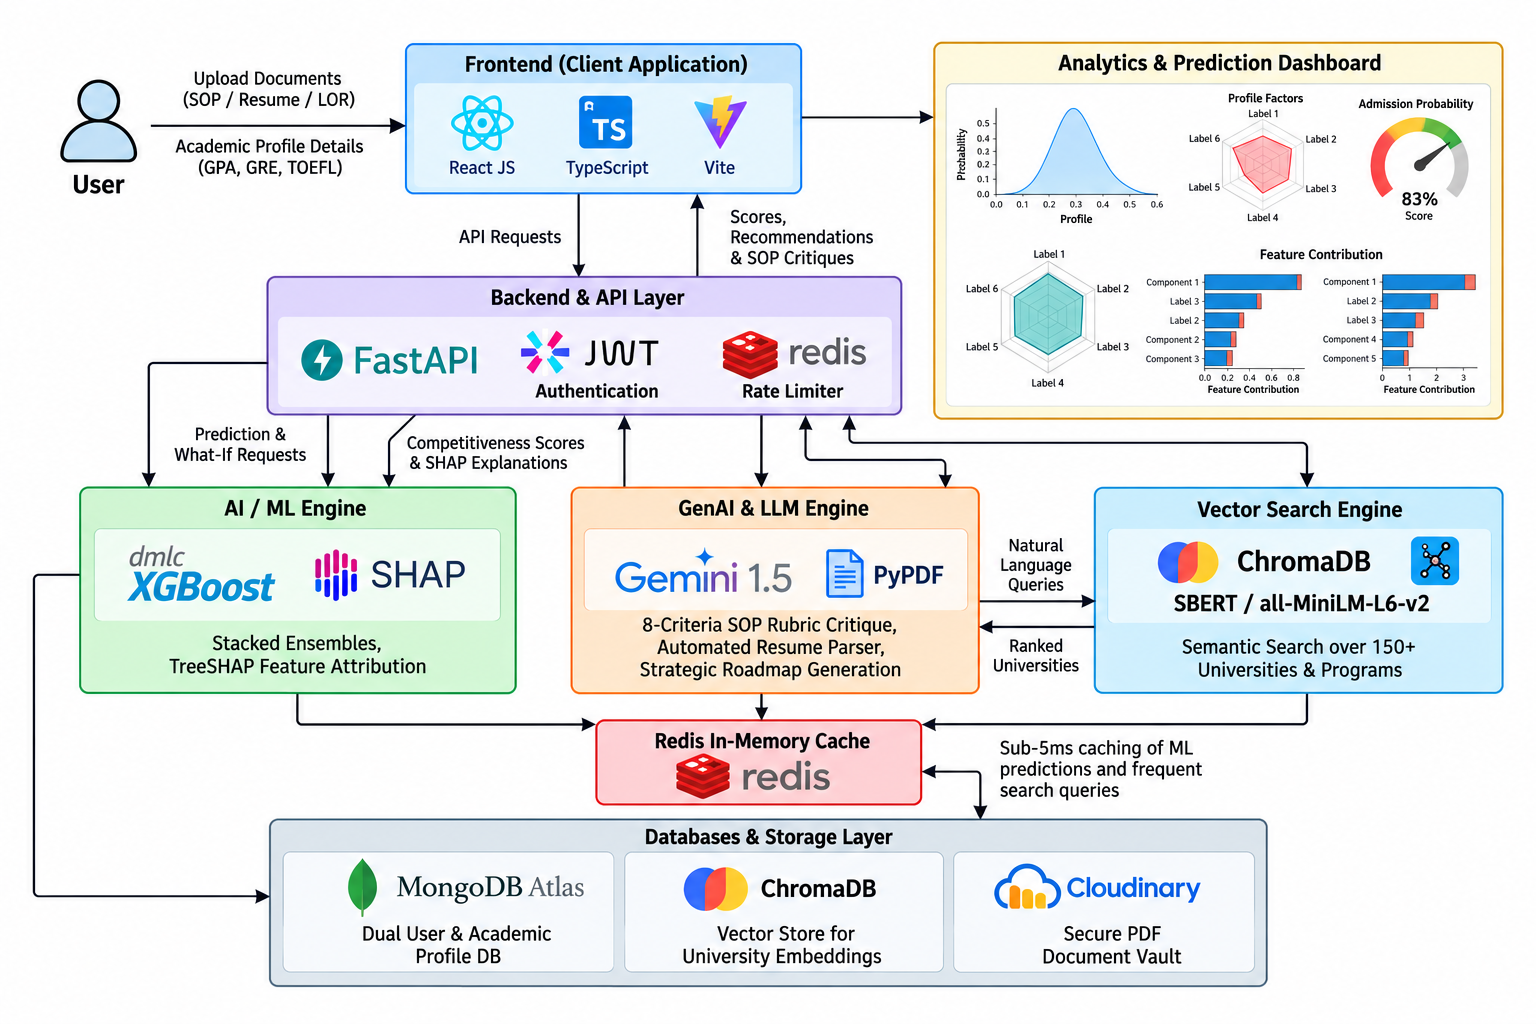
\includegraphics[width=\columnwidth]{System_Arch.png}
    \caption{ML Model Architecture: Ensemble Stacking and Explainability}
    \label{fig:ml_model_architecture}
\end{figure}

Figure~\ref{fig:ml_model_architecture} illustrates the ensemble 
stacking architecture of the proposed admission prediction model, 
integrating four base classifiers with five-fold cross-validation 
and a Logistic Regression meta-classifier to predict admission 
probabilities. SHAP TreeExplainer provides feature attribution 
values, improving the interpretability and transparency of the 
model's predictions.




%------------------------------------------------
% Comparative Model Evaluation
%------------------------------------------------

\subsection{Comparative Model Performance Evaluation}

All candidate models were evaluated on the held-out test set
($N = 11{,}655$) using ROC-AUC, accuracy, precision, recall,
F1-score, and Brier score. These metrics assess classification
performance and probabilistic prediction quality. A lower Brier
score indicates better probabilistic accuracy.



%------------------------------------------------
% Discussion and Key Observations
%------------------------------------------------

\subsection{Discussion and Key Observations}

\begin{enumerate}

    \item \textbf{Superior Overall Performance:}
    The stacking ensemble achieved the highest ROC-AUC of 0.8465,
    outperforming XGBoost (0.8418) and the Logistic Regression
    baseline (0.7412). Its accuracy of 76.26\% and F1-score of
    0.7896 further support its selection as the production model.

    \item \textbf{Recall and Applicant Guidance:}
    The ensemble achieved a recall of 0.8130 (81.30\%), indicating
    that it identified a substantial proportion of positive cases
    in the test set. Recall is relevant because false-negative
    predictions may cause applicants to overlook potentially
    suitable opportunities.

    \item \textbf{Probabilistic Prediction Quality:}
    The ensemble recorded the lowest Brier score (0.1593) among
    the evaluated models. Further calibration analysis would help
    assess how closely predicted probabilities correspond to
    observed outcomes.

\end{enumerate}

The results demonstrate that the stacking ensemble achieved the
best overall performance among the evaluated models, based on
the reported classification and probabilistic metrics.

%------------------------------------------------
% Comparative Model Performance Table
%------------------------------------------------

\begin{table}[!htbp]
\centering
\caption{Comparative Performance of Candidate Models}
\label{tab:model_performance}

\scriptsize
\setlength{\tabcolsep}{3pt}
\renewcommand{\arraystretch}{1.15}

\resizebox{\columnwidth}{!}{%
\begin{tabular}{lcccccc}
\toprule
\textbf{Model Architecture} &
\textbf{ROC-AUC} &
\textbf{Accuracy (\%)} &
\textbf{Precision} &
\textbf{Recall} &
\textbf{F1-Score} &
\textbf{Brier Score} \\
\midrule
Logistic Regression (Baseline) & 0.7412 & 68.45 & 0.6910 & 0.7320 & 0.7109 & 0.2084 \\
Random Forest (150 Trees) & 0.8190 & 73.82 & 0.7431 & 0.7850 & 0.7635 & 0.1742 \\
Extra Trees (Bagging) & 0.8124 & 73.15 & 0.7380 & 0.7794 & 0.7581 & 0.1789 \\
LightGBM (Leaf-Wise Boosted) & 0.8389 & 75.40 & 0.7588 & 0.8045 & 0.7810 & 0.1631 \\
XGBoost (Optimized Trees) & 0.8418 & 75.85 & 0.7625 & 0.8090 & 0.7851 & 0.1610 \\
\textbf{Stacking Ensemble (Meta-Learner)} &
\textbf{0.8465} & \textbf{76.26} & \textbf{0.7674} &
\textbf{0.8130} & \textbf{0.7896} & \textbf{0.1593} \\
\bottomrule
\end{tabular}%
}
\end{table}

\vspace{10pt}


The stacking
ensemble achieved the highest ROC-AUC (0.8465) and accuracy
(76.26\%), while recording the lowest Brier score (0.1593)
among the evaluated models.

\end{table*}


%------------------------------------------------
% Continue with the next section here
%------------------------------------------------


\vspace{30pt}
\justify
This chapter presented the results and discussion of the MsAdmit system, including its user interfaces, key functionalities, core algorithms, and testing procedures. It described the implementation of admission prediction, TreeSHAP explainability, SOP evaluation, semantic university search, and what-if simulations. The testing results and comparative model evaluation demonstrated the functionality of the tested components, with the stacking ensemble achieving the highest ROC-AUC of 0.8465 and an accuracy of 76.26\% among the evaluated models.

% Chapter 10 Conclusion

\chapter{Conclusion \& Future Scope} \label{chap6}
\newpage

\justify
\section{Conclusion} \label{sec:6.1}
\subsection{Summary}


MsAdmit is an AI-powered platform designed to help students planning to pursue higher education abroad make informed admission decisions. It evaluates students' academic profiles, test scores, skills, and other achievements to assess their admission competitiveness and recommend suitable universities under three categories: Reach, Target, and Consider.

The platform uses machine learning and Explainable AI to generate personalized recommendations and identify areas for improvement. Additional features, such as resume parsing, SOP evaluation, a what-if simulator, and application tracking, help students prepare their applications and manage important deadlines. By integrating these features into a single platform, MsAdmit aims to make the admission process more organized, transparent, and accessible.
\subsection{Conclusion}
MsAdmit offers a structured approach to the challenges students face when applying to graduate programs abroad. By combining AI-based profile evaluation, university recommendations, and application management tools, the platform helps students understand their strengths, identify areas for improvement, and plan their applications more effectively.

This project demonstrates how artificial intelligence and machine learning can support personalized educational guidance. Although the recommendations cannot guarantee admission, they can help students make more informed decisions. 
\justify

\section{Future Scope} \label{sec:6.2}

    

\begin{itemize}
    \item \textbf{Real-Time Data Synchronization:} Automated web scraping pipelines and university API connectors will be integrated for continuous real time tracking of admission deadlines, tuition updates, cohort acceptance rates, and GRE waiver policies.

    \item \textbf{Multidisciplinary Expansion:} The predictive modeling and recommendation engine will be expanded beyond Computer Science to support different fields including Business Administration (MBA), Biomedical Sciences, and Humanities.

    \item \textbf{LOR and Transcript Intelligence:} Advanced document evaluation models will be integrated to analyze Letter of Recommendation (LOR) depth, referee alignment, and academic transcript precondition matching.

    \item \textbf{Scholarship and Funding Matcher:} Automated financial advisory algorithms will be incorporated to connect applicant profiles with departmental research/teaching assistantships (RA/TA) and global merit based fellowships.

    \item \textbf{Covering more Number of Universities:} At present, the system covers the top 150 QS ranked universities for Computer Science and IT. In future, this coverage can be extended to the top 500 universities worldwide. 
\end{itemize}
% End of Chapter

%\addcontentsline{toc}{chapter}{\bibname}





% =========================================================
% REFERENCES
% =========================================================
\clearpage
\renewcommand{\bibname}{References}
\addcontentsline{toc}{chapter}{References}

\bibliographystyle{ieeetr}
\bibliography{hypnosis}







\addcontentsline{toc}{chapter}{Acknowledgement}
% Acknowledgment Page

\begin{centering}
    \large
{\LARGE\bf Acknowledgement}\\
\end{centering}
    
\justify
The success of a project like this, involving high technical expertise, patience, and massive support from guides, is possible when team members work together. We take this opportunity to express our gratitude to those who have been instrumental in the successful completion of this project. We would like to show our appreciation to \textbf{Dr. Chhaya Pawar} for their tremendous support and help; without them, this project would not have reached fruition. We would also like to thank our project coordinator \textbf{Dr. Rakhi Kalantri} for providing us with regular inputs about documentation and project timeline. A big thanks to our HOD \textbf{Dr. M.Kiruthika } for all the encouragement given to our team. We would also like to thank our principal, \textbf{Dr. S. M. Khot}, and our college, \textbf{Fr. C. Rodrigues Institute of Technology, Vashi}, for giving us the opportunity and the environment to learn and grow.

\vspace{3cm}
\hfill% move it to the right
\begin{tabular}[t]{l@{}}
\vspace{1cm}

{\textbf{Project Group Members:}} \\ 
\vspace{1cm}

1. Samiksha Khandagale, 1023151 \\
\noindent\rule{5cm}{0.10pt} \\
\\
\vspace{1cm}

2. Shivangi Khandelwal, 1023152 \\
\noindent\rule{5cm}{0.10pt} \\
\\
\vspace{1cm}

3. Shubham Khilari, 1023153 \\
 \noindent\rule{5cm}{0.10pt}
\\
\\
\vspace{1cm}

4. Racheal Kodiyan, 1023154 \\
 \noindent\rule{5cm}{0.10pt}
\\
\vspace{2cm}
\end{tabular}
%%%%%%%%%%%%%%%%%%%%%%%%%%%%%%%%%%%%
%\begin{flushright} 
%\vspace{0.5in}
%\noindent\rule{4cm}{0.4pt} \\ (Signature)\\
%\vspace{0.3in}
%\noindent\rule{4cm}{0.4pt} \\ (Name of the Student)
%\end{flushright}
%\vspace{0.5cm}
%{\bf Date:} \\
%%%%%%%%%%%%%%%%%%%%%%%%%%%%%%%%%%%%
%% End of Acknowledgement Page



%\addcontentsline{toc}{chapter}{Acknowledgement}
%\include{92Acknowledgment}
\addcontentsline{toc}{chapter}{Appendix A: Timeline Chart}
% Fun Fact :- Only way to add vertical spacing in lateX is to use \vspace* coz \vspace is deleted if it is at the beginning. Use it wisely

\vspace*{5cm}
\begin{centering}
    \large
{\LARGE\bf Appendix A : Timeline Chart}\\
\end{centering}





% Add this in the preamble


\begin{figure}[htbp]
    \centering
    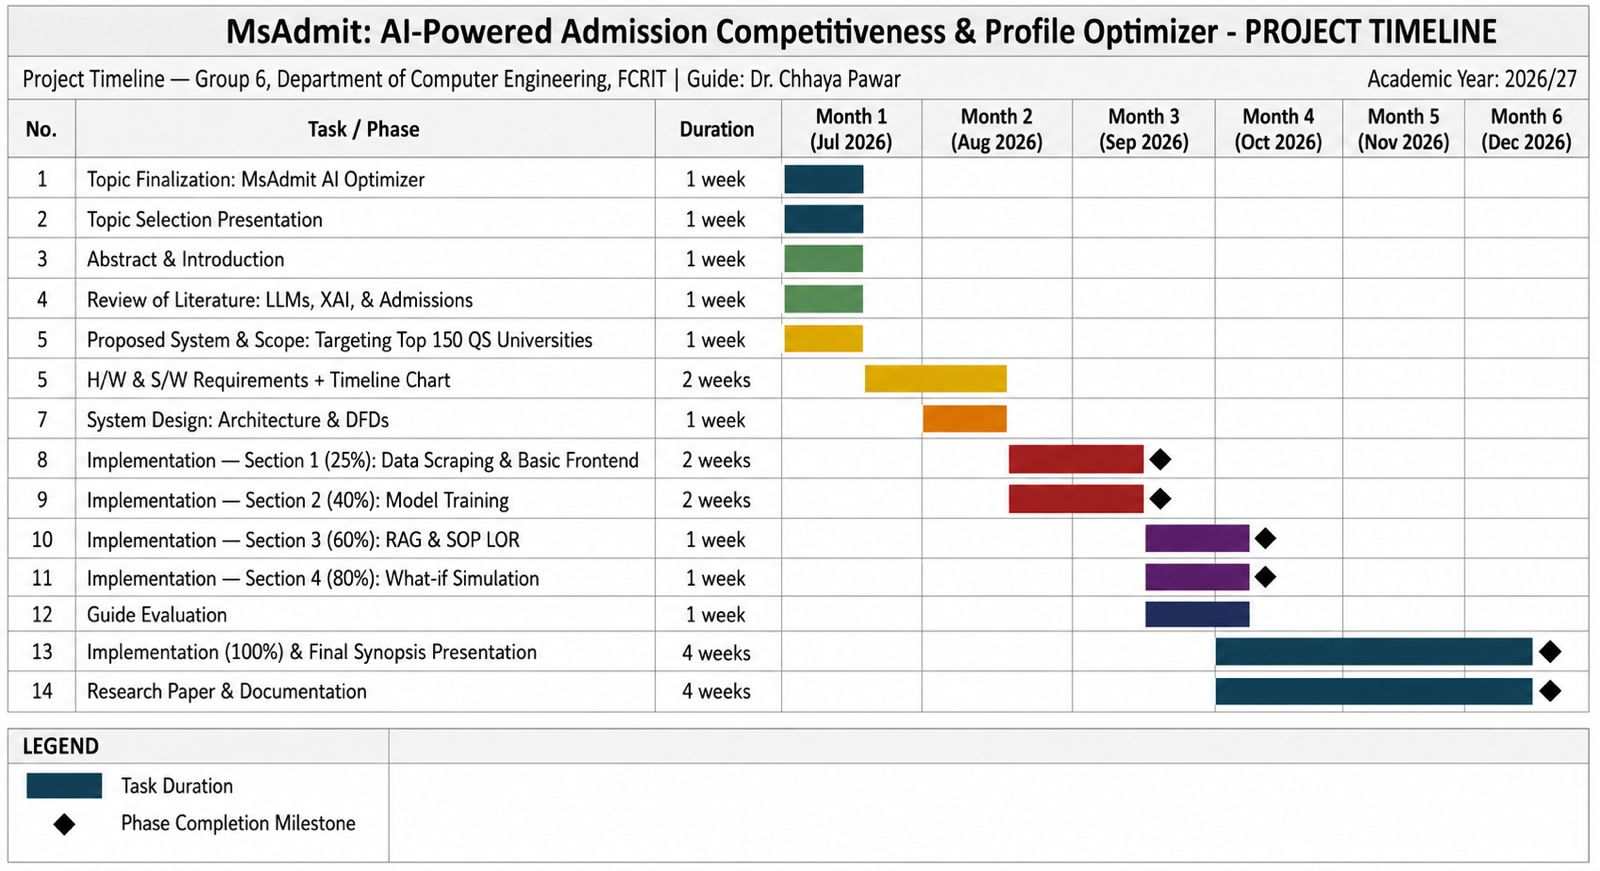
\includegraphics[width=\textwidth]{timeline_1.jpeg}
    \caption*{\textbf{Timeline Chart of the Project Development}}
    \label{fig:timeline}
\end{figure}

\newpage
\addcontentsline{toc}{chapter}{Appendix B: Sustainable Development Goal (SDG) Mapping}
\chapter*{Appendix B}

\label{app:sdg_mapping}

The project team has identified the following Sustainable Development Goal(s) (SDG) relevant to the proposed project. The mapping should demonstrate a clear and meaningful relationship between the project problem, proposed solution, and the selected SDG(s).

\vspace{0.4cm}

\begin{center}
\textbf{\large SDG Mapping of the Project}
\end{center}

\vspace{0.3cm}

%------------------------------------------------
% SDG Mapping Table
%------------------------------------------------

\renewcommand{\arraystretch}{1.4}

\begin{center}
\begin{tabular}{|c|c|p{4.2cm}|p{6.0cm}|}
\hline
\textbf{Sr. No.} &
\textbf{SDG No.} &
\textbf{Complete Name of SDG} &
\textbf{Rationale / Contribution of the Project} \\
\hline

1 &
4 &
\parbox[t]{4.2cm}{
\vspace{0.15cm}
Quality Education
\vspace{1.4cm}
} &
\parbox[t]{6.0cm}{
\vspace{0.15cm}
MsAdmit promotes accessible and personalized graduate admission guidance by helping students assess their profiles, identify suitable universities, and understand areas for improvement, supporting informed decisions about higher education.
\vspace{1.4cm}
}
\\
\hline





\end{tabular}
\end{center}

\vspace{0.5cm}

%------------------------------------------------
% Guidelines
%------------------------------------------------



\vspace{1.0cm}

%------------------------------------------------
% Guide Verification
%------------------------------------------------

\begin{center}

\rule{6cm}{0.2px}\\
\textbf{Signature of Project Guide}\\[0.4cm]

Name of Project Guide: \rule{5cm}{0.2px}\\[0.4cm]

Date: \rule{3cm}{0.2px}

\end{center}


\addcontentsline{toc}{chapter}{Appendix C: Complex Engineering Problem Identification and Evaluation}
%=========================================================
% APPENDIX C
% COMPLEX ENGINEERING PROBLEM IDENTIFICATION AND EVALUATION
%=========================================================

\chapter*{Appendix C}

{Appendix C: Complex Engineering Problem Identification and Evaluation}

\begin{center}
    {\Large\bfseries COMPLEX ENGINEERING PROBLEM}\\[0.15cm]
    {\Large\bfseries IDENTIFICATION AND EVALUATION}
\end{center}

\vspace{0.3cm}

\noindent
The Washington Accord emphasizes the ability of engineering graduates
to identify, analyse and solve complex engineering problems using
appropriate engineering knowledge, modern tools, multidisciplinary
thinking and analytical reasoning. The Major Project provides an
opportunity for students to demonstrate these abilities through a
structured and evidence-based project.

\vspace{0.25cm}

\noindent
This appendix provides a structured mechanism to assess the complexity
of the proposed Major Project. The assessment is initially carried out
by the student team and subsequently verified by the Project Guide.

%---------------------------------------------------------
% A. PROJECT DETAILS
%---------------------------------------------------------


\section*{A. Project Details}

\begin{center}
\renewcommand{\arraystretch}{1.4}

\begin{tabular}{|p{5cm}|p{9cm}|}
\hline
\textbf{Project Title} & MsAdmit: AI-Powered Admission Competitiveness and Profile Optimizer \\[0.5cm]
\hline
\textbf{Group / Team No.} & Group 6 \\[0.4cm]
\hline
\textbf{Name of Student(s)} & Samiksha Khandagale , Shivangi Khandelwal , Shubham Khilari , Racheal Kodiyan  \\[0.7cm]
\hline
\textbf{Project Guide} & Dr. Chhaya Pawar \\[0.4cm]
\hline
\textbf{Academic Year} & 2026--2027 \\[0.4cm]
\hline
\end{tabular}

\end{center}




%---------------------------------------------------------
% B. COMPLEXITY EVALUATION
%---------------------------------------------------------

\section*{B. Complexity Evaluation}

\noindent
For each parameter, the student team shall assign a score from
\textbf{0 to 3} and provide a suitable justification or evidence.
The Project Guide shall review the student's assessment and record
the verified score in the final column.

\vspace{0.3cm}

\begin{center}

\small
\renewcommand{\arraystretch}{1.35}

\begin{tabularx}{\textwidth}{|
>{\centering\arraybackslash}p{0.7cm}|
p{3.8cm}|
>{\centering\arraybackslash}p{1.1cm}|
X|
>{\centering\arraybackslash}p{1.1cm}|}

\hline

\textbf{Sr. No.} &
\textbf{Complexity Parameter} &
\textbf{Student Score} &
\textbf{Student Justification / Evidence} &
\textbf{Guide Score} \\

\hline

1 &
Problem novelty and research depth &
&
&
\\[0.8cm]

\hline

2 &
Multidisciplinary knowledge requirement &
&
&
\\[0.8cm]

\hline

3 &
System design complexity &
&
&
\\[0.8cm]

\hline

4 &
Technology integration &
&
&
\\[0.8cm]

\hline

5 &
Data analysis and experimentation &
&
&
\\[0.8cm]

\hline

6 &
Societal / industrial relevance &
&
&
\\[0.8cm]

\hline

7 &
Stakeholder involvement &
&
&
\\[0.8cm]

\hline

8 &
Sustainability considerations &
&
&
\\[0.8cm]

\hline

\multicolumn{2}{|r|}{\textbf{Total Score}} &
\textbf{/24} &
&
\textbf{/24} \\

\hline

\end{tabularx}

\end{center}

%---------------------------------------------------------
% SCORING GUIDELINE
%---------------------------------------------------------

\vspace{0.3cm}

\noindent
\textbf{Scoring Guideline}

\vspace{0.1cm}

\begin{center}

\renewcommand{\arraystretch}{1.25}

\begin{tabular}{|c|p{8.5cm}|}
\hline
\textbf{Score} & \textbf{Interpretation} \\
\hline
0 & Not applicable / negligible \\
\hline
1 & Basic level of complexity \\
\hline
2 & Moderate level of complexity \\
\hline
3 & Significant / high level of complexity \\
\hline
\end{tabular}

\end{center}

\vspace{0.3cm}

\noindent
\textbf{Maximum Score: 24}

%---------------------------------------------------------
% C. FINAL PROJECT CLASSIFICATION
%---------------------------------------------------------
\newpage
\section*{C. Final Project Classification}

\noindent
The final classification shall be based on the score verified by the
Project Guide.

\vspace{0.25cm}

\begin{center}

\renewcommand{\arraystretch}{1.4}

\begin{tabular}{|c|p{6.5cm}|}
\hline
\textbf{Score Range} & \textbf{Project Classification} \\
\hline
0--8 & Simple Engineering Problem \\
\hline
9--16 & Moderately Complex Engineering Problem \\
\hline
17--24 & Complex Engineering Problem \\
\hline
\end{tabular}

\end{center}

\vspace{0.35cm}

\noindent
\textbf{Final Classification:}

\vspace{0.15cm}

\noindent
$\square$ Simple Engineering Problem

\vspace{0.15cm}

\noindent
$\square$ Moderately Complex Engineering Problem

\vspace{0.15cm}

\noindent
$\square$ Complex Engineering Problem

%---------------------------------------------------------
% D. GUIDE'S FINAL REMARKS
%---------------------------------------------------------


\centering
\textbf{Project Guide Signature}
\\[0.8cm]

\centering
Date: \rule{3cm}{0.4pt}



%=========================================================
% END OF APPENDIX C
%=========================================================
\addcontentsline{toc}{chapter}{Appendix D: Project Outcomes}
\include{appendixD}

\end{document}


